\documentclass[12pt,paper=A4,english,headings=small,footlines=2.1,footheight=15mm]{scrreprt}
\def\execdate{07.11.2023}
\def\docsubject{Laboratory protocol\\Fundamentals of signal processing}
\def\authors{Franz Linden (101052) \\ Kaan Tali (943588)}
\def\docauthor{Franz Linden (101052) \\ Kaan Tali (943588) \\ \\ Technische Informatik – Embedded Systems (B.Eng.)}
\def\docdate{Winter semester 2023/2024\\\execdate}
\def\docpublishers{Prof.~Dr.~P.~Gregorius}

\usepackage[english]{babel}
\usepackage[utf8]{inputenc}
\usepackage[export]{adjustbox}
\usepackage[
	a4paper,
	includeheadfoot,
	top=0mm,
	tmargin=15mm,
	right=25mm,
	bottom=10mm,
	left=20mm,
	marginpar=0mm,
	marginparwidth=0mm,
	marginparsep=0mm,
	headheight=15mm,
	footskip=20mm,
]{geometry}
\usepackage{refcount}
\usepackage{lastpage}
\usepackage{microtype}

\usepackage[headsepline, footsepline]{scrlayer-scrpage}
\clearpairofpagestyles

\renewcommand*{\headfont}{\normalfont}
\ihead[\authors]{\authors}
\ohead[\doctitle]{\doctitle}
\ifoot[\docdate]{\docdate}
\ofoot[\pagemark]{\pagemark}
\ofoot{Page \thepage\ of \pageref{LastPage}}
\renewcommand*\chapterpagestyle{scrheadings}% default pagestyle on chapter pages is plain

\ModifyLayer[addvoffset=-.6ex]{scrheadings.foot.above.line}
\ModifyLayer[addvoffset=-.6ex]{plain.scrheadings.foot.above.line}

% Schriftart
\usepackage{libertine}
\usepackage{libertinust1math}
\usepackage[T1]{fontenc}
\setlength{\parindent}{0pt}
\usepackage{accents}
\usepackage{moresize}

% Mathe, Symbole, Einheitendarstellung, Chemie
\usepackage{amsmath}
\usepackage{amsxtra}
\usepackage{amssymb}
\usepackage{siunitx}
\DeclareSIUnit \voltampere { VA } %apparent power 
\DeclareSIUnit \var { var } %volt-ampere reactive - idle power 
\sisetup{locale=DE}
\usepackage{gauss}
\usepackage{mathtools}
\DeclarePairedDelimiter\abs{\lvert}{\rvert}
\usepackage{cancel}

% Layout
\usepackage{enumitem}
\usepackage{float}
\usepackage{graphicx}
\usepackage{multirow,multicol,booktabs}
\usepackage{tabularx}
\usepackage[hidelinks,
colorlinks,
linkcolor={black},
citecolor={blue!50!black},
urlcolor={blue!80!black}]{hyperref}
\urlstyle{rm}
\usepackage[table]{xcolor}
\newcommand{\ccgray}{\cellcolor[HTML]{dddddd}}
\newcolumntype{R}{>{\raggedleft\arraybackslash}X}
\newcolumntype{L}{>{\raggedright\arraybackslash}X}
\usepackage{wrapfig}
\usepackage{pgfplots}
\usepgfplotslibrary{polar, fillbetween}
\pgfplotsset{compat=newest}
\usetikzlibrary{arrows, shapes.symbols, shapes.geometric, angles,quotes, intersections, backgrounds}
\usepgfplotslibrary{groupplots}
\usepackage[european,siunitx]{circuitikz}
\usepackage{circuitikz}
\ctikzset{bipoles/thickness=1}
\tikzset{>=latex} % for LaTeX arrow head
\usepackage{caption}

\usepackage{listings} % codepackage

% Übergreifende Zählung von figures auch bei chapter wechsel
\usepackage{chngcntr}
\counterwithout{figure}{chapter}

\RedeclareSectionCommand[beforeskip=0pt, afterskip=6pt]{chapter}
\RedeclareSectionCommand[beforeskip=6pt, afterskip=6pt]{section}


\usepackage{xparse}

% Redefine \vec environment to be bold+upright instead of arrow
\let\vec\mathbf

% Matlab format
\definecolor{codegreen}{rgb}{0,0.6,0}
\definecolor{codegray}{rgb}{0.5,0.5,0.5}
\definecolor{codepurple}{rgb}{0.58,0,0.82}
\definecolor{backcolor}{rgb}{0.95,0.95,0.95}

\lstdefinestyle{matlab}{
	backgroundcolor=\color{backcolor},
	commentstyle=\color{codegreen},
	keywordstyle=\color{magenta},
	numberstyle=\tiny\color{codegray},
	stringstyle=\color{codepurple},
	breakatwhitespace=false,
	breaklines=true,
	captionpos=b,
	keepspaces=true,
	numbers=left,
	numbersep=5pt,
	showspaces=false,
	showstringspaces=false,
	showtabs=false,
	tabsize=2,
	inputencoding=utf8,
	extendedchars=true,
	texcl=true,
	%	basicstyle=\ttfamily\footnotesize,
	basicstyle=\scriptsize
}
\lstset{
style=matlab,
literate=%
	{Ö}{{\"O}}1
{Ä}{{\"A}}1
{Ü}{{\"U}}1
{ß}{{\ss}}1
{ü}{{\"u}}1
{ä}{{\"a}}1
{ö}{{\"o}}1
}

\newcommand\inlcode[2]{
	\fontsize{10}{10}\texttt{\color{magenta}#1(\color{codepurple}#2\color{magenta})}
}

% wrapper around \includegraphics with a colored box
\newcommand{\addimg}[2][backcolor]{%
	\setlength{\fboxsep}{0pt}%
	\colorbox{#1}{\includegraphics[width=\linewidth, keepaspectratio]{#2}}%
}

% Footnote without number
\newcommand\nnfootnote[1]{%
	\begingroup
	\renewcommand\thefootnote{}\footnote{#1}%
	\addtocounter{footnote}{-1}%
	\endgroup
	%	\vspace{-pt}%
}

\newcommand{\rme}{\ensuremath{\mathrm{e}}}
\newcommand{\dunderline}[1]{
	\underline{\underline{#1}}
}
\newcommand{\D}[1]{\ensuremath{
		\;\mathrm{d}{#1}
	}}

% Debug
%\usepackage{showframe}
%\renewcommand\ShowFrameLinethickness{0.15pt}
%\renewcommand*\ShowFrameColor{\color{red}}
%\showboxbreadth=\maxdimen
%\showboxdepth=\maxdimen

% Remove several warnings
\usepackage{scrhack} % Overcome differentiating floats from KOMA and other like lstlisting
\usepackage{silence}
\WarningFilter{scrreprt}{Usage of package `fancyhdr'} % fancyhdr with KOMA
\def\doctitle{Laboratory I\\Introduction to Matlab/Octave and signal theory}

\begin{document}

% Title
\thispagestyle{plain}
\titlehead{
	\vspace*{-2cm}
	\begin{multicols}{2}
		\raggedcolumns
		\text{Berliner Hochschule für Technik}\\
		\text{Fachbereich VI -- Informatik und Medien}
		\columnbreak
		
\includegraphics[width=6cm, right]{../BHT_Logo.png} % Path relative to main.tex
	\end{multicols}
}

\subject{\docsubject}
\title{\doctitle}
\author{\docauthor}
\date{\docdate}

\publishers{\docpublishers}

\maketitle

\pagenumbering{arabic}
\tableofcontents

\cleardoublepage

\chapter{Vectors and matrices (3.3)}

\section{Scalar multiplied with vector (3.3.1)}
Given are the following vectors:
\begin{align*}
	\vec{x}&=\begin{pmatrix}
		\frac{1}{16} \\ \frac{2}{7} \\ 3
	\end{pmatrix} &
	\vec{y}&=\begin{pmatrix}
		4 \\ 5 \\ 6
	\end{pmatrix}
\end{align*}
and the scalar:
\begin{align*}
	\alpha = \frac{1}{5}
\end{align*}

Calculations should be performed for:
\begin{align*}
	\vec{z}_1&=\alpha\cdot\vec{x} & \vec{z}_2&=\alpha\cdot\vec{x}^T \\
	\vec{w}_1&=\alpha\cdot\vec{y} & \vec{w}_2&=\alpha\cdot\vec{y}^T
\end{align*}

\subsubsection{Solution}
{
	\setlength{\abovedisplayskip}{0pt}
	\setlength{\belowdisplayskip}{6pt}
	\setlength{\abovedisplayshortskip}{0pt}
	\setlength{\belowdisplayshortskip}{0pt}
	\begin{flalign*}
		&\vec{z}_1 =\alpha\cdot\vec{x} = \frac{1}{5} 
		\cdot \begin{pmatrix}
			\frac{1}{16} \\ \frac{2}{7} \\ 3
		\end{pmatrix} 
		= \begin{pmatrix}
			\frac{1}{5}\cdot\frac{1}{16} \\ \frac{1}{5}\cdot\frac{2}{7} \\ \frac{1}{5}\cdot3
		\end{pmatrix} 
		= \begin{pmatrix}
			\frac{1}{80} \\ \frac{2}{35} \\
			\frac{3}{5}
		\end{pmatrix} &
	\end{flalign*}
	
	\begin{flalign*}
		&\vec{z}_2 =\alpha\cdot\vec{x}^T = \frac{1}{5} 
		\cdot \begin{pmatrix}
			\frac{1}{16} & \frac{2}{7} & 3
		\end{pmatrix} 
		= \begin{pmatrix}
			\frac{1}{5}\cdot\frac{1}{16} & \frac{1}{5}\cdot\frac{2}{7} & \frac{1}{5}\cdot3
		\end{pmatrix} 
		= \begin{pmatrix}
			\frac{1}{80} & \frac{2}{35} & \frac{3}{5}
		\end{pmatrix} &
	\end{flalign*}
	\begin{flalign*}
		&\vec{w}_1 =\alpha\cdot\vec{y} = \frac{1}{5} 
		\cdot \begin{pmatrix}
			4 \\ 5 \\ 6
		\end{pmatrix} 
		= \begin{pmatrix}
			\frac{1}{5}\cdot4 \\ \frac{1}{5}\cdot5 \\ \frac{1}{5}\cdot6
		\end{pmatrix} 
		= \begin{pmatrix}
			\frac{4}{5} \\ \frac{5}{5} \\ \frac{6}{5}
		\end{pmatrix}
		= \begin{pmatrix}
			\frac{4}{5} \\ 1 \\	\frac{6}{5}
		\end{pmatrix} &
	\end{flalign*}
	\begin{flalign*}
		&\vec{w}_2 =\alpha\cdot\vec{y}^T = \frac{1}{5} 
		\cdot \begin{pmatrix}
			4 & 5 & 6
		\end{pmatrix} 
		= \begin{pmatrix}
			\frac{1}{5}\cdot4 & \frac{1}{5}\cdot5 & \frac{1}{5}\cdot6
		\end{pmatrix}
		= \begin{pmatrix}
			\frac{4}{5} & \frac{5}{5} & \frac{6}{5}
		\end{pmatrix}
		= \begin{pmatrix}
			\frac{4}{5} & 1 & \frac{6}{5}
		\end{pmatrix} &
	\end{flalign*}
}

\subsubsection{Matlab}
\lstinputlisting[language=Matlab]{./assets/Lab1_331.m}

Output
\lstinputlisting{./assets/Lab1_331o.txt}
\vspace{20pt}



\section{Vector multiplied with vector (3.3.2)}
Given are the following vectors:
\begin{align*}
	\vec{x}&=\begin{pmatrix}
		\frac{1}{16} \\ \frac{2}{7} \\ 3
	\end{pmatrix} &
	\vec{y}&=\begin{pmatrix}
		4 \\ 5 \\ 6
	\end{pmatrix}
\end{align*}

Calculations should be performed for:
\begin{align*}
	\vec{z}_1&=\vec{x}.\cdot\vec{y} & \vec{z}_2&=\vec{x}^T\cdot\vec{y} & \vec{z}_3&=\vec{x}\cdot\vec{y}^T
\end{align*}

\subsubsection{Solution}
{
	\setlength{\abovedisplayskip}{0pt}
	\setlength{\belowdisplayskip}{6pt}
	\setlength{\abovedisplayshortskip}{0pt}
	\setlength{\belowdisplayshortskip}{0pt}
	\begin{flalign*}
		&\vec{z}_1=\vec{x}.\cdot\vec{y}=\begin{pmatrix}
			\frac{1}{16} \\ \frac{2}{7} \\ 3
		\end{pmatrix}\cdot\begin{pmatrix}
			4 \\ 5 \\ 6
		\end{pmatrix}=\begin{pmatrix}
		\frac{1}{16} \cdot 4  \\ \frac{2}{7} \cdot 5 \\ 3 \cdot 6
		\end{pmatrix}=\begin{pmatrix}
		\frac{4}{16} \\ \frac{10}{7} \\ 18
		\end{pmatrix}=\begin{pmatrix}
		\frac{1}{4} \\ \frac{10}{7} \\ 18
		\end{pmatrix}&
	\end{flalign*}
	
	\begin{flalign*}
		& \vec{z}_2=\vec{x}^T\cdot\vec{y} = \begin{pmatrix}
			\frac{1}{16} & \frac{2}{7} & 3
		\end{pmatrix}\cdot\begin{pmatrix}
		4 \\ 5 \\ 6
		\end{pmatrix}= \begin{pmatrix}
		\frac{1}{16}\cdot4 + \frac{2}{7}\cdot5 + 3\cdot6
		\end{pmatrix}=\begin{pmatrix}\num{19,68}\end{pmatrix}& 
	\end{flalign*}
	
	
	\begin{flalign*}
		& \vec{z}_3=\vec{x}\cdot\vec{y}^T = \begin{pmatrix}
			\frac{1}{16} \\ \frac{2}{7} \\ 3
		\end{pmatrix}\cdot\begin{pmatrix}
			4 & 5 & 6
		\end{pmatrix}= 
		\begin{pmatrix}
			\frac{1}{16}\cdot4 & \frac{1}{16}\cdot5 & \frac{1}{16}\cdot6 \\
			\frac{2}{7}\cdot4 & \frac{2}{7}\cdot5 & \frac{2}{7}\cdot6 \\
			3\cdot4 & 3\cdot5 & 3\cdot6
		\end{pmatrix}=
		\begin{pmatrix}
			\frac{4}{16} & \frac{5}{16} & \frac{6}{16}  \\
			\frac{8}{7} & \frac{10}{7} & \frac{12}{7}  \\
			12 & 15 & 18
		\end{pmatrix}=
		\begin{pmatrix}
			\frac{1}{4} & \frac{5}{16} & \frac{3}{8}  \\
			\frac{8}{7} & \frac{10}{7} & \frac{12}{7}  \\
			12 & 15 & 18
		\end{pmatrix}& 
	\end{flalign*}
}

\clearpage

\subsubsection{Matlab}
\lstinputlisting[language=Matlab]{./assets/Lab1_332.m}

Output
\lstinputlisting{./assets/Lab1_332o.txt}
\vspace{20pt}

\section{Vector multiplied with matrix - A (3.3.3)}
Given are the following vector and matrix:
\begin{align*}
	\vec{x}&=\begin{pmatrix}
		1 \\ 2 \\ 3
	\end{pmatrix} &
	\vec{Y}&=\begin{pmatrix}
		1 & 4 \\
		2 & 5 \\
		3 & 6
	\end{pmatrix}
\end{align*}

Calculations should be performed for:
\begin{align*}
	\vec{Z}=\vec{x}^T\cdot{Y}
\end{align*}

\subsubsection{Solution}
{
	\setlength{\abovedisplayskip}{0pt}
	\setlength{\belowdisplayskip}{6pt}
	\setlength{\abovedisplayshortskip}{0pt}
	\setlength{\belowdisplayshortskip}{0pt}	
	\begin{flalign*}
		\vec{Z}& =\vec{x}^T\cdot{Y} = \vec{x}=\begin{pmatrix}
			1 & 2 & 3
		\end{pmatrix}\cdot\begin{pmatrix}
			1 & 4 \\
			2 & 5 \\
			3 & 6
		\end{pmatrix}=\begin{pmatrix}
			1\cdot1+2\cdot2+3\cdot3 &
			1\cdot4+2\cdot5+3\cdot6
		\end{pmatrix}&\\
		&=\begin{pmatrix}
			14 & 32\end{pmatrix}& 
	\end{flalign*}
}

\subsubsection{Matlab}
\lstinputlisting[language=Matlab]{./assets/Lab1_333.m}

Output
\lstinputlisting{./assets/Lab1_333o.txt}
\vspace{20pt}

\section{Vector multiplied with matrix - B (3.3.4)}
Given are the following vector and matrix:
\begin{align*}
	\vec{x}&=\begin{pmatrix}
		+\frac{1}{2}+j\frac{1}{2} \\
		-\frac{1}{2}-j\frac{1}{2} \\
		+\frac{1}{2}-j\frac{1}{2}
	\end{pmatrix} &
	\vec{Y}&=\begin{pmatrix}
		1 & 4 \\
		2 & 5 \\
		3 & 6
	\end{pmatrix}
\end{align*}

Calculations should be performed for:
\begin{align*}
	\vec{Z}=\vec{x}^T\cdot{Y}
\end{align*}

\subsubsection{Solution}
{
	\setlength{\abovedisplayskip}{0pt}
	\setlength{\belowdisplayskip}{6pt}
	\setlength{\abovedisplayshortskip}{0pt}
	\setlength{\belowdisplayshortskip}{0pt}	
	\begin{flalign*}
		\vec{Z}&=\vec{x}^T\cdot{Y} =\begin{pmatrix}
			+\frac{1}{2}+j\frac{1}{2} &
			-\frac{1}{2}-j\frac{1}{2} &
			+\frac{1}{2}-j\frac{1}{2}
		\end{pmatrix}\cdot\begin{pmatrix}
			1 & 4 \\
			2 & 5 \\
			3 & 6
		\end{pmatrix}& \\
		&=\begin{pmatrix}
			\left(\frac{1}{2}+j\frac{1}{2}\right) \cdot 1 +
			\left(-\frac{1}{2}-j\frac{1}{2}\right) \cdot 2 +
			\left(\frac{1}{2}-j\frac{1}{2}\right) \cdot 3 &
			\left(\frac{1}{2}+j\frac{1}{2}\right) \cdot 4 +
			\left(-\frac{1}{2}-j\frac{1}{2}\right) \cdot 5 +
			\left(\frac{1}{2}-j\frac{1}{2}\right) \cdot 6 
		\end{pmatrix} & \\ 
		&=\begin{pmatrix}
		\left(\frac{1}{2}+j\frac{1}{2}\right)
		+\left(-1-j\right)
		+\left(\frac{3}{2}-j\frac{3}{2}\right) &&
		\left(2+j2\right)
		+\left(-\frac{5}{2}-j\frac{5}{2}\right)
		+\left(3-j3\right)
		\end{pmatrix} & \\ 
		&=\begin{pmatrix}
			1-j2 & \frac{5}{2}-j\frac{7}{2}
		\end{pmatrix}
		=\begin{pmatrix}
			1-2j & \num{2,5}-\num{3,5}j
		\end{pmatrix}&
	\end{flalign*}
}

\subsubsection{Matlab}
\lstinputlisting[language=Matlab]{./assets/Lab1_334.m}

Output
\lstinputlisting{./assets/Lab1_334o.txt}

\chapter{Signal display and characteristic values (4.1)}

\section{Continuous signals (4.1.1)}
Given is the continuous signal:
{
	\setlength{\abovedisplayskip}{0pt}
	\setlength{\belowdisplayskip}{6pt}
	\setlength{\abovedisplayshortskip}{0pt}
	\setlength{\belowdisplayshortskip}{0pt}
	\begin{align*}
		s(t) = \cos\left[{\omega_0\cdot\left(t-\tau_0\right)+\theta_0}\right]
	\end{align*}
}
\renewcommand{\labelenumi}{\alph{enumi})}

\newenvironment{nscenter}
{\parskip=0pt\par\nopagebreak\centering}
{\par\noindent\ignorespacesafterend}
\begin{enumerate}
	\item
		Calculation of the frequency and period duration, as well as representation of the signal curves for the cases:
		\begin{nscenter}
			\begin{tabular}{c|lll}
				& $\omega_0$ & $\tau_0$ & $\theta_0$ \\
				\hline
				1 & $\pi/3$ & $0$ & $2\pi$ \\
				2 & $3\pi/4$ & $1/2$ & $\pi/{4}$ \\
				3 & $3/4$ & $1/2$ & $1/4$ \\
			\end{tabular}
		\end{nscenter}
		
		\subsubsection{General information}
		The frequency $f$, defined as the number of oscillations within a unit of time, given in $\si{\Hz} = 1\fracslash\si{\s}$. In general, the frequency is described by the quotient of wave speed $c$ and wavelength $\lambda$. Alternatively, it can also be derived using the circular frequency $\omega$. This is based on the assumption that a complete oscillation on a circle of $2\pi$ requires exactly one frequency.
		{
			\setlength{\abovedisplayskip}{0pt}
			\setlength{\belowdisplayskip}{6pt}
			\setlength{\abovedisplayshortskip}{0pt}
			\setlength{\belowdisplayshortskip}{0pt}
			\begin{align*}
				\omega = 2\pi{f} \rightarrow f = \frac{\omega}{2\pi}
			\end{align*}
		}%
		The period duration $T$ indicates the time required to complete a full oscillation. From this follows formally
		{
			\setlength{\abovedisplayskip}{0pt}
			\setlength{\belowdisplayskip}{6pt}
			\setlength{\abovedisplayshortskip}{0pt}
			\setlength{\belowdisplayshortskip}{0pt}
			\begin{align*}
				T = \frac{1}{f}
			\end{align*}
		}
		
		\subsubsection{Solution}
		{
			\setlength{\abovedisplayskip}{0pt}
			\setlength{\belowdisplayskip}{6pt}
			\setlength{\abovedisplayshortskip}{0pt}
			\setlength{\belowdisplayshortskip}{0pt}
			\sisetup{parse-numbers=false}
			\begin{flalign*}
				&f_1 = \frac{\frac{\pi}{3}}{2\pi} = \frac{\pi}{3\cdot{2}\pi} = \SI{\frac{1}{6}}{\Hz} &
				&T_1 = \frac{1}{\frac{1}{6}} = \SI{\frac{6}{1}}{\s} = \SI{6}{\s} & \\
				%
				&f_2 = \frac{\frac{3\pi}{4}}{2\pi} = \frac{3\pi}{{4}\cdot2\pi} = \SI{\frac{3}{8}}{\Hz} & 
				&T_2 = \frac{1}{\frac{3}{8}} =  \SI{\frac{8}{3}}{\s} \approx \SI{2,6\overline{6}}{\s} & \\
				%
				&f_3 = \frac{\frac{3}{4}}{2\pi} = \frac{3}{4\cdot2\pi} = \SI{\frac{3}{8\pi}}{\Hz} \approx \SI{0,12}{\Hz} & 
				&T_3 = \frac{1}{\frac{3}{8\pi}} = \SI{\frac{8\pi}{3}}{\s} \approx \SI{8,38}{\s} & 
			\end{flalign*}
			
			Signal curves\newline
			The signal curves $s_n(t)$, are drawn in the interval $0 \leq t \leq 4\pi$.
			
			\pgfplotsset{
				axis411a/.style={
					xlabel=$t$,
					x label style={at={(current axis.right of origin)},	anchor=east, right=1mm},
					y label style={at={(current axis.above origin)}, anchor=south }
				},
			}
			
			\begin{tikzpicture}
				\begin{groupplot}
					[
						group style={
							group size=1 by 3,
							xlabels at=edge bottom,
							ylabels at=edge left,
							horizontal sep=0.2\textwidth, group name=plots,
						},
						width=\linewidth,
						height=4cm,
						ylabel=$s$,
						ymin=-1.1, ymax=1.1,
						ytick={-1,-0.5,0,0.5,1},
						axis x line=middle,
						axis y line=center,
						tick align=outside,
						hide obscured y ticks=false,
						grid=both,
						grid style={line width=.1pt, draw=gray!10},
						major grid style={line width=.2pt,draw=gray!30},
						ytick distance = 1,
						xtick={-2*pi, -(3*pi)/2, -pi, -pi/2, pi/2, pi, (3*pi)/2, 2*pi, (5*pi)/2, 3*pi, (7*pi)/2, 4*pi},
						xticklabels={$-2\pi$, $-\frac{3\pi}{2}$, $-\pi$, $-\frac{\pi}{2}$, $\frac{\pi}{2}$, $\pi$, $\frac{3\pi}{2}$, $2\pi$, $\frac{5\pi}{2}$, $3\pi$, $\frac{7\pi}{2}$, $4\pi$ },
						domain=0:4*pi+0.2
					]
					\nextgroupplot[title=$s_1(t)$, axis411a]
					\addplot [samples=500,color=blue] {cos(deg((pi/3)*(x-0) + 2*pi))};
					
					\nextgroupplot[title=$s_2(t)$, axis411a]
					\addplot [samples=500,color=red] {cos(deg((3*pi/4)*(x-(1/2)) + (pi/4)))};
					
					\nextgroupplot[title=$s_3(t)$, axis411a]
					\addplot [samples=500,color=orange] {cos(deg((3/4)*(x-(1/2)) + (1/4)))};
				\end{groupplot}
			\end{tikzpicture}
		}
		\subsubsection{Matlab}
		\lstinputlisting[language=Matlab]{./assets/Lab1_411a.m}
		
		Output
		\lstinputlisting{./assets/Lab1_411ao.txt}
		Signal curves
		
		{
			\setlength{\fboxsep}{0pt}%  
			\colorbox{backcolor}{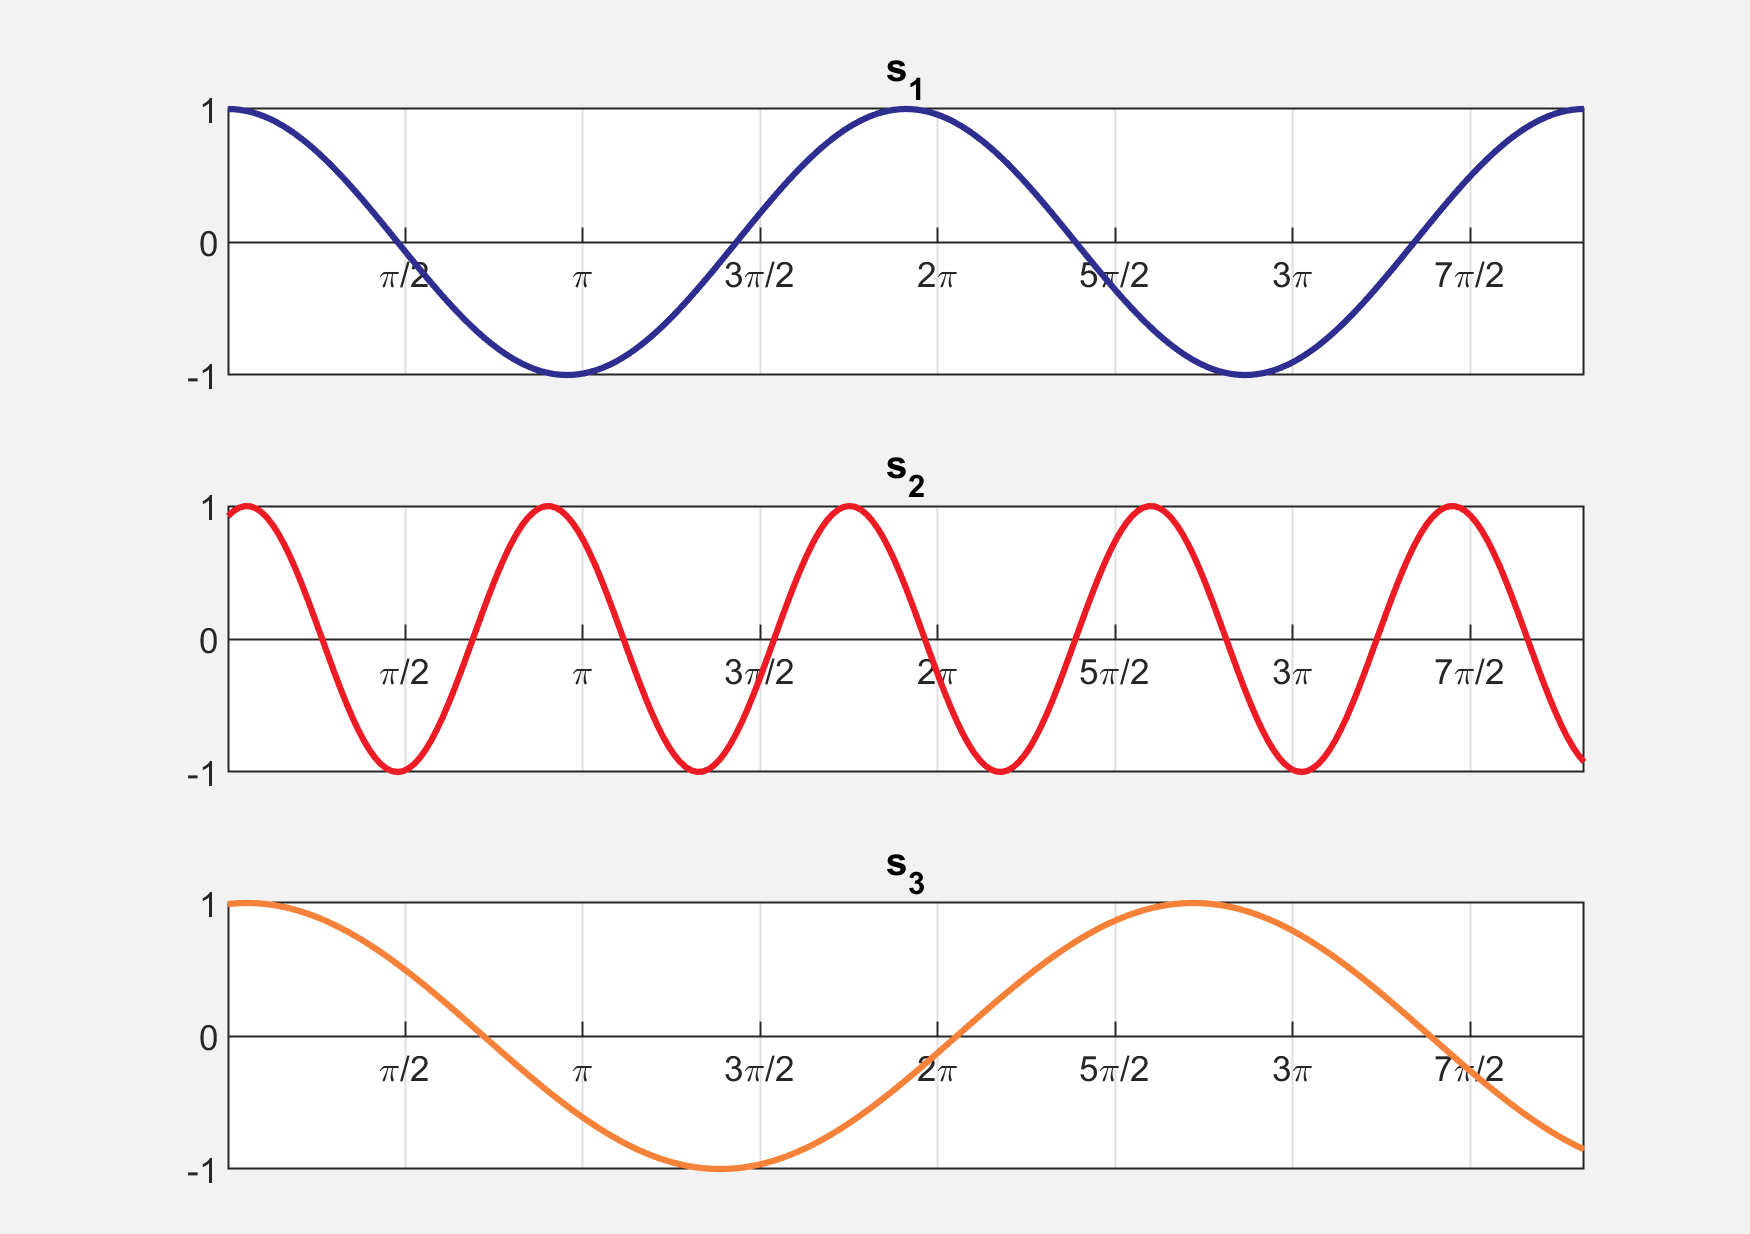
\includegraphics[width=0.9\linewidth, keepaspectratio]{./assets/411a.png}}
		}
		
	\item 
		Given are the signals:
		{
			\setlength{\abovedisplayskip}{0pt}
			\setlength{\belowdisplayskip}{6pt}
			\setlength{\abovedisplayshortskip}{0pt}
			\setlength{\belowdisplayshortskip}{0pt}
			\begin{align*}
				s_1(t) = \cos\left[{\omega_x\cdot\left(t-\tau_x\right)+\theta_x}\right] \\
				s_2(t) = \sin\left[{\omega_y\cdot\left(t-\tau_y\right)+\theta_y}\right]
			\end{align*}
		}
		and the parameters:
		
		\begin{nscenter}
			\begin{tabular}{c|lll|lll}
				& $\omega_x$ & $\tau_x$ & $\theta_x$ & $\omega_y$ & $\tau_y$ & $\theta_y$ \\
				\hline
				1 & $\pi/{3}$ & $0$ & $2\pi$ & $\pi/3$ & $1$ & $-7\pi/6$ \\
				2 & $3\pi/4$ & $1/2$ & $\pi/4$ & $11\pi/4$ & $1$ & $3\pi/8$ \\
				3 & $3/4$ & $1/2$ & $1/4$ & $3/4$ & $1$ & $13/8$ \\
			\end{tabular}
		\end{nscenter}\\
		This gives us the functions:
		{
			\setlength{\abovedisplayskip}{0pt}
			\setlength{\belowdisplayskip}{6pt}
			\setlength{\abovedisplayshortskip}{0pt}
			\setlength{\belowdisplayshortskip}{0pt}
			\begin{align*}
				s_{11}(t) = \cos\left[\frac{\pi}{3}\cdot\left(t-0\right)+2\pi\right] & \qquad 
				s_{21}(t) = \sin\left[\frac{\pi}{3}\cdot\left(t-1\right)-\frac{7\pi}{6}\right] \\
				%
				s_{12}(t) = \cos\left[\frac{3\pi}{4}\cdot\left(t-\frac{1}{2}\right)+\frac{\pi}{4}\right] & \qquad 
				s_{22}(t) = \sin\left[\frac{11\pi}{4}\cdot\left(t-1\right)+\frac{3\pi}{8}\right] \\
				%
				s_{13}(t) = \cos\left[\frac{3}{4}\cdot\left(t-\frac{1}{2}\right)+\frac{1}{4}\right] & \qquad 
				s_{23}(t) = \sin\left[\frac{3}{4}\cdot\left(t-1\right)+\frac{13}{8}\right]
			\end{align*}
		}
		\subsubsection{Solution}
		It is to be checked for which of the given combinations $s_{1i}(t)$ is identical to $s_{2i}(t)$. \\
		Since sine and cosine have a phase shift of $\SI{90}{\degree}$ ($\pi/2$) to each other, a cosine function can be converted into a sine function by adding this shift. \vspace{2pt}
		{
			\setlength{\abovedisplayskip}{0pt}
			\setlength{\belowdisplayskip}{6pt}
			\setlength{\abovedisplayshortskip}{0pt}
			\setlength{\belowdisplayshortskip}{0pt}
			
			\underline{Signal combination 1:}
			
			\begin{minipage}[t]{0.499999\linewidth}
				\begin{flalign*}
					s_{11}(t) & = \cos\left[\frac{\pi}{3}\cdot\left(t-0\right)+2\pi\right] & \\
					&=\cos\left(\frac{\pi}{3}t\right) & \\
					&=\sin\left(\frac{\pi}{3}t + \frac{\pi}{2}\right) &
				\end{flalign*}
			\end{minipage}
			\begin{minipage}[t]{0.499999\linewidth}
				\begin{flalign*}
					s_{21}(t) & = \sin\left[\frac{\pi}{3}\cdot\left(t-1\right)-\frac{7\pi}{6}\right] & \\
					&=\sin\left(\frac{\pi}{3}t - \frac{\pi}{3} - \frac{\pi}{3}\right) & \\
					&=\sin\left(\frac{\pi}{3}t - \frac{2\pi}{3}\right) &
				\end{flalign*}
			\end{minipage}
			\vspace{2pt} \\
			$\Rightarrow$ The signals have the same frequency of $\pi/3$ and amplitude of $1$, but a phase shift to each other of $\SI{30}{\degree}$, $\pi/6$ (shift on the x-axis).
			
			\vspace{4pt}
			\clearpage
			\underline{Signal combination 2:}
			
			\begin{minipage}[t]{0.499999\linewidth}
				\begin{flalign*}
					s_{12}(t) & = \cos\left[\frac{3\pi}{4}\cdot\left(t-\frac{1}{2}\right)+\frac{\pi}{4}\right] & \\
					&=\cos\left(\frac{3\pi}{4}t - \frac{3\pi}{8} + \frac{\pi}{4} \right) & \\
					&=\cos\left(\frac{3\pi}{4}t - \frac{\pi}{8}\right) & \\
					&=\sin\left(\frac{3\pi}{4}t - \frac{\pi}{8} + \frac{\pi}{2}\right) & \\
					&=\sin\left(\frac{3\pi}{4}t + \frac{3\pi}{8}\right) &
				\end{flalign*}
			\end{minipage}
			\begin{minipage}[t]{0.499999\linewidth}
				\begin{flalign*}
					s_{22}(t) & = \sin\left[\frac{11\pi}{4}\cdot\left(t-1\right)+\frac{3\pi}{8}\right] & \\
					&=\sin\left(\frac{11\pi}{4}t - \frac{11\pi}{4}+\frac{3\pi}{8}\right) & \\
					&=\sin\left(\frac{11\pi}{4}t - \frac{19\pi}{8}\right) &
				\end{flalign*}
			\end{minipage}
			\vspace{2pt} \\
			$\Rightarrow$ The signals only have the same amplitude.	
			
			\vspace{4pt}
			\underline{Signal combination 3:}
			
			\begin{minipage}[t]{0.499999\linewidth}
				\begin{flalign*}
					s_{13}(t) & = \cos\left[\frac{3}{4}\cdot\left(t-\frac{1}{2}\right)+\frac{1}{4}\right] & \\
					&=\cos\left(\frac{3\pi}{4}t - \frac{3}{8} + \frac{1}{4}\right) & \\
					&=\cos\left(\frac{3\pi}{4}t - \frac{1}{8}\right) & \\
					&=\sin\left(\frac{\pi}{3}t - \frac{1}{8} + \frac{\pi}{2}\right) &
				\end{flalign*}
			\end{minipage}
			\begin{minipage}[t]{0.5\linewidth}
				\begin{flalign*}
					s_{23}(t) & = \sin\left[\frac{3}{4}\cdot\left(t-1\right)+\frac{13}{8}\right] & \\
					&=\sin\left(\frac{3}{4}t - \frac{3}{4} + \frac{13}{8}\right) & \\
					&=\sin\left(\frac{\pi}{3}t + \frac{7}{8}\right) &
				\end{flalign*}
			\end{minipage}
			\vspace{2pt} \\
			$\Rightarrow$ As in the first combination, these two signals are also identical in terms of frequency and amplitude. However, they have a phase shift of $\SI{2,33}{\radian}$ in relation to each other.
		}
		
		\subsubsection{Matlab}
		\lstinputlisting[language=Matlab]{./assets/Lab1_411b.m}
		Signal curves\newline
		{
			\setlength{\fboxsep}{0pt}%  
			\colorbox{backcolor}{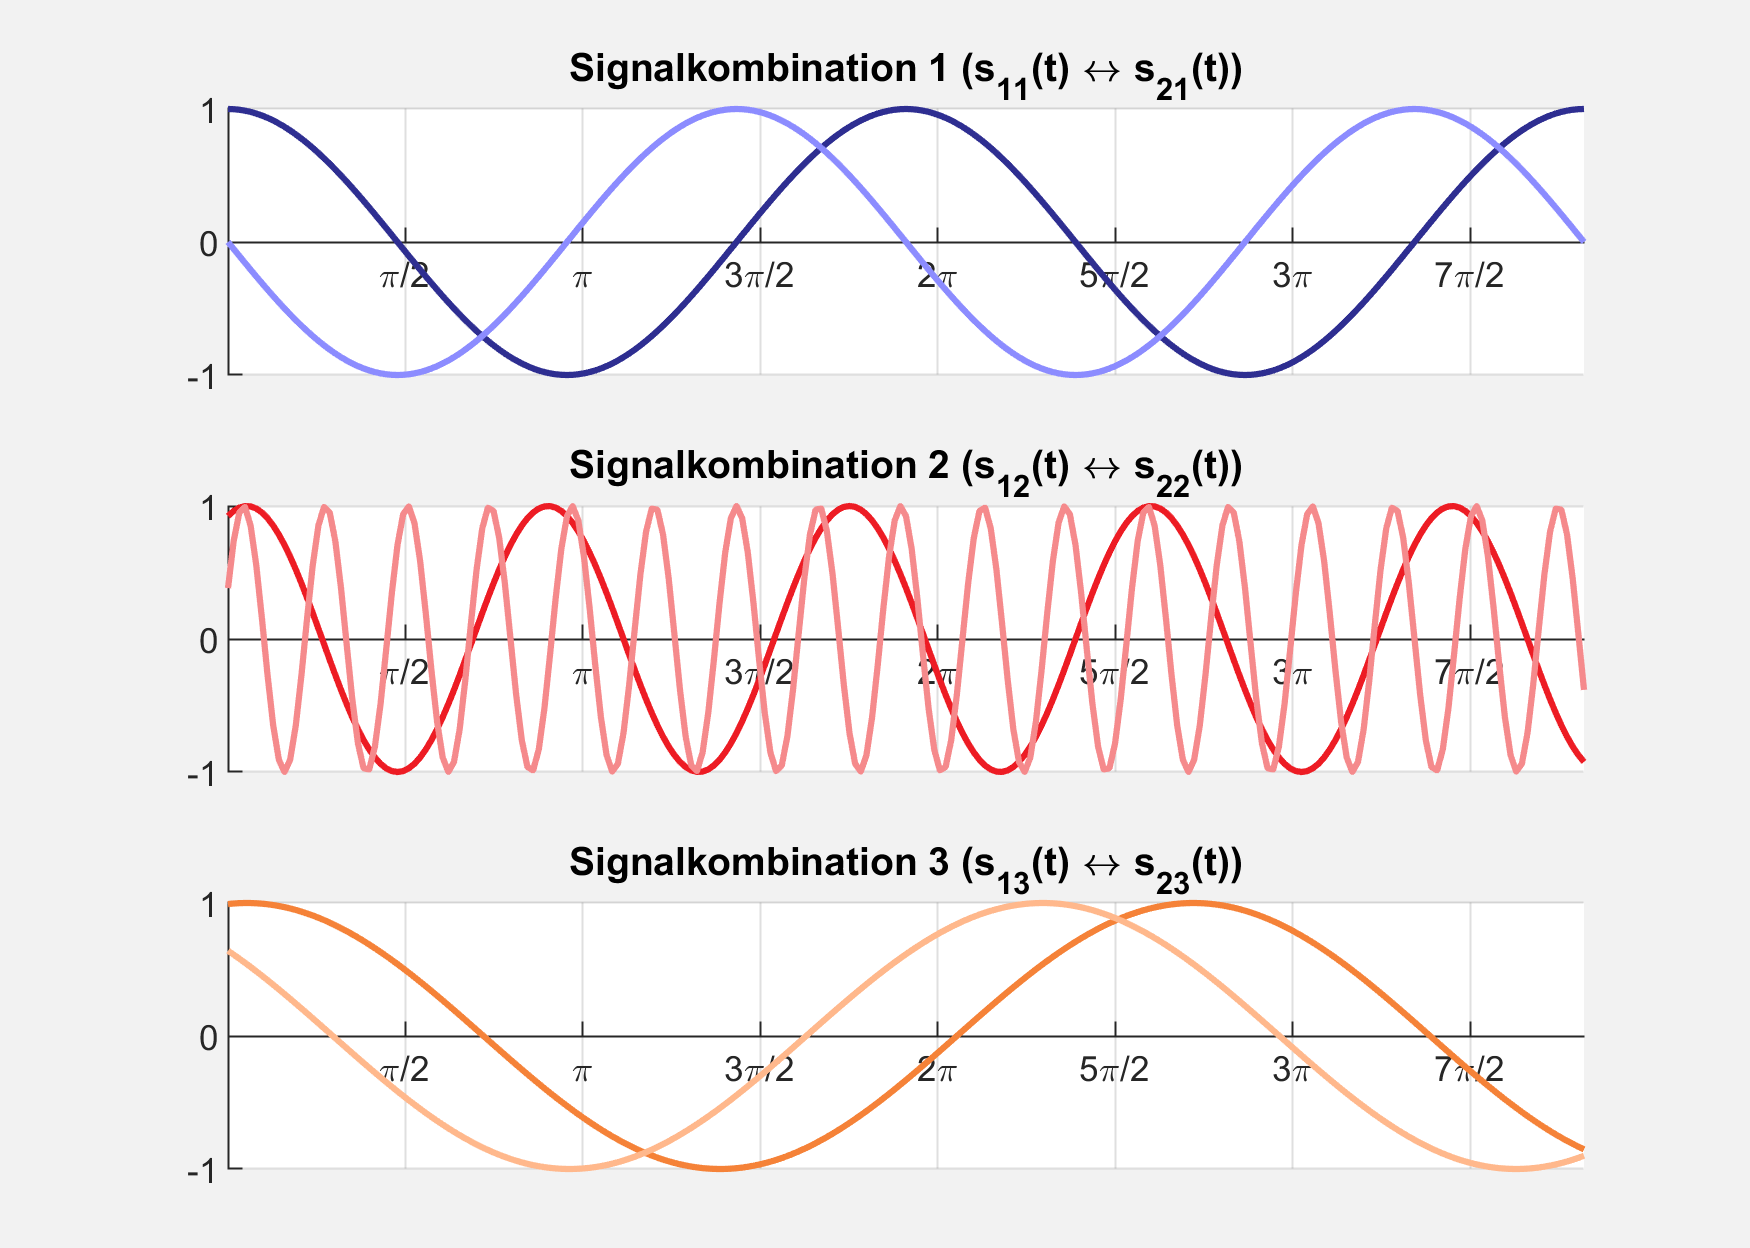
\includegraphics[width=\linewidth, keepaspectratio]{./assets/411b.png}}
		}
\end{enumerate}
\clearpage

\section{Simple continuous signals (4.1.2)}
Given is the continuous signal $s(t)$.

\pgfplotsset{
	axis412/.style={
			clip=false,
			axis lines=middle,
			xmin=-6.5, xmax=6.5,
			xlabel={$t$},
			xtick distance={2},
			ymin=0, ymax=1.3,
			y=2.5cm,
			ylabel={$s(t)$},
			yticklabels={$\hat{s}$},
			ytick={1},
			hide obscured x ticks=false,
			x label style={at={(current axis.right of origin)},	anchor=east, right=1mm},
			y label style={at={(current axis.above origin)}, anchor=south },
			hide obscured x ticks=false
		},
}

\begin{figure}[H]
	\centering
	\begin{tikzpicture}
		\pgfplotsset{
			every axis plot/.append style={line width=1pt, mark=none, samples=10}
		}
		\begin{axis}[axis412,width=12cm, xtick distance={1}]
			\addplot[color=blue] coordinates {(-6,0) (0,0) (0,1) (3,0) (6,0)};
			\addplot[color=gray!60, line width=0.75pt, dashed] coordinates {(0,1) (3,1)  (3,0)};

			\draw node[above] at (1.5, 1) {$3$};
			\draw node[right] at (3, 0.5) {$1$};
		\end{axis}
	\end{tikzpicture}
	\caption{\label{412-1}$s(t)$}
\end{figure}

If $\hat{s} = 1$, the following applies to $s(t)$
\begin{flalign*}
	\quad s(t) = \begin{cases}
		             0, \quad t < 0                     \\
		             \hat{s}=1, \quad t = 0             \\
		             -\frac{1}{3}t + 1, \quad 0 < t < 3 \\
		             0, \quad t > 3
	             \end{cases}
\end{flalign*}

\subsubsection{Solutions}
\begin{tabularx}{\linewidth}{@{}l@{}X@{}@{}l@{}X@{}}
	a)                                &
	\begin{equation*}
		s(-t) = \begin{cases}
			0, \quad t > 0                     \\
			\hat{s}=1, \quad t = 0             \\
			\frac{1}{3}t + 1, \quad -3 < t < 0 \\
			0, \quad t < -3
		\end{cases}
	\end{equation*} &
	b)                                &
	\begin{equation*}
		s(t+2) = \begin{cases}
			0, \quad t < -2                               \\
			\hat{s}=1, \quad t = -2                       \\
			-\frac{1}{3}t + \frac{1}{3}, \quad -2 < t < 1 \\
			0, \quad t \geq 1
		\end{cases}
	\end{equation*}   \\
	                                  &
	\begin{tikzpicture}
		\begin{axis}[axis412]
			\addplot[color=blue] coordinates {(-6,0) (-3,0) (0,1) (0,0) (6,0)};
		\end{axis}
	\end{tikzpicture}         &

	                                  &
	\begin{tikzpicture}
		\begin{axis}[axis412]
			\addplot[color=blue] coordinates {(-6,0) (-2,0) (-2,1) (1,0) (6,0)};
		\end{axis}
	\end{tikzpicture}
\end{tabularx}

\begin{tabularx}{\linewidth}{@{}l@{}X@{}@{}l@{}X@{}}
	c)                                  &
	\begin{equation*}
		s(2t+2) = \begin{cases}
			0, \quad t < -1                                         \\
			\hat{s}=1, \quad t = -1                                 \\
			-\frac{2}{3}t + \frac{1}{3}, \quad -1 < t < \frac{1}{2} \\
			0, \quad t \geq \frac{1}{2}
		\end{cases}
	\end{equation*} &
	d)                                  &
	\begin{equation*}
		s(1-3t) = \begin{cases}
			0, \quad t \leq -\frac{2}{3}                           \\
			t+\frac{2}{3}, \quad -\frac{2}{3} \leq t < \frac{1}{3} \\
			\hat{s}=1, \quad t = \frac{1}{3}                       \\
			0, \quad t \geq \frac{1}{3}
		\end{cases}
	\end{equation*}    \\
	                                    &
	\begin{tikzpicture}
		\begin{axis}[axis412]
			\addplot[color=blue] coordinates {(-6,0) (-1,0) (-1,1) (1/2,0) (6,0)};
		\end{axis}
	\end{tikzpicture}          &
	                                    &
	\begin{tikzpicture}
		\begin{axis}[axis412]
			\addplot[color=blue] coordinates {(-6,0) (-2/3,0) (1/3,1) (1/3,0) (6,0)};
		\end{axis}
	\end{tikzpicture}
\end{tabularx}

\subsubsection{Matlab}
\lstinputlisting[language=Matlab]{./assets/Lab1_412.m}
{
	\setlength{\fboxsep}{0pt}%  
	\colorbox{backcolor}{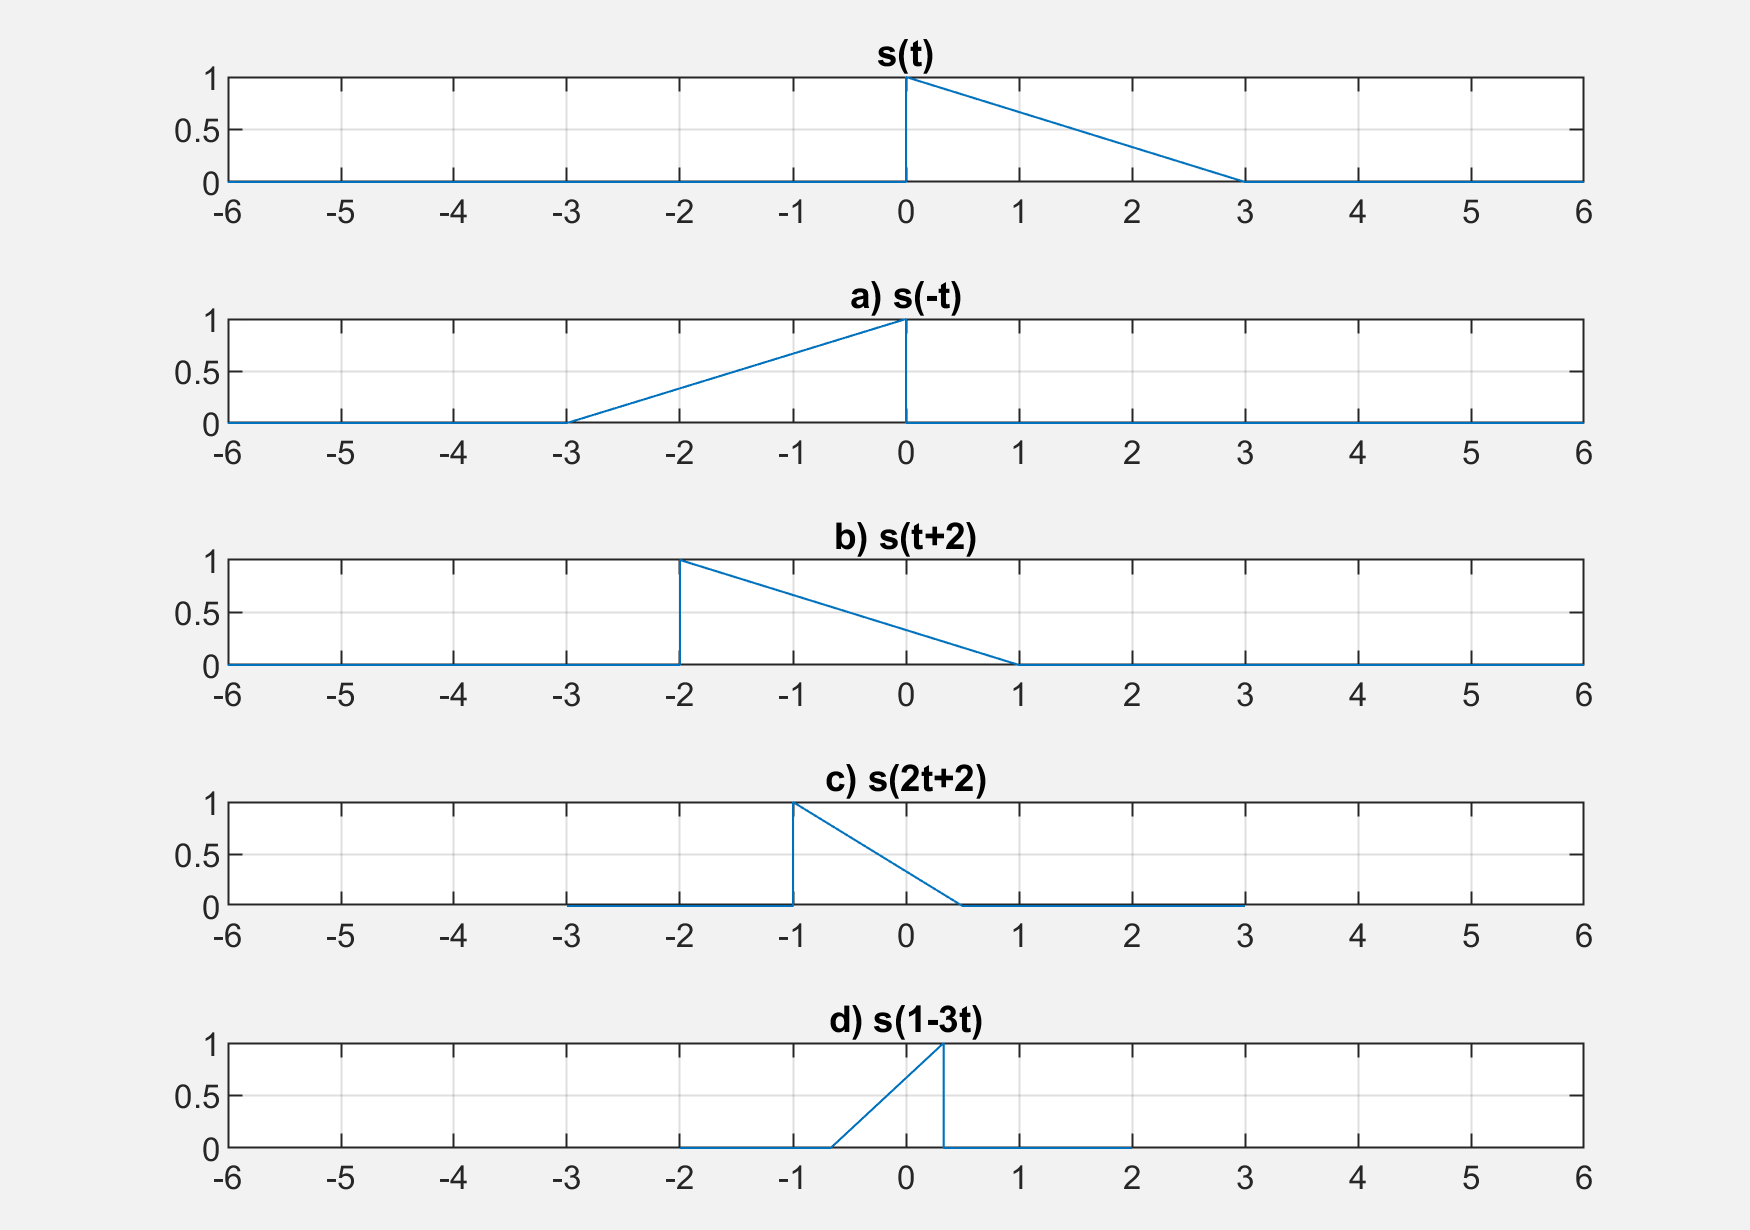
\includegraphics[width=\linewidth, keepaspectratio]{./assets/412.png}}
}

\section{Even and odd signals (4.1.3)}
The signals $s_1(t)$ and $s_2(t)$ are given. It is to be checked whether these signals are even or odd.
\pgfplotsset{
	axis413/.style={
		clip=false,
		axis lines=middle,
		xmin=-6.5, xmax=6.5,
		xlabel={$t$},
		x label style={at={(current axis.right of origin)},	anchor=east, right=1mm},
		xtick distance={1},
		ymin=0, ymax=1.3,
		y=2.5cm,
		ylabel={$s(t)$},
		y label style={at={(current axis.above origin)}, anchor=south },
		yticklabels={$\hat{s}$ = -1, $\hat{s}$ = 1},
		ytick={-1,1},
		hide obscured x ticks=false,
	},
}
\begin{figure}[H]
	\centering
	\begin{tikzpicture}
		\begin{groupplot}[			
			group style={
				group size=1 by 2,
				xlabels at=edge bottom,
				ylabels at=edge left,
				vertical sep=+48pt, group name=plots,
			},
			width=0.8\linewidth,
		]
			\pgfplotsset{
				every axis plot/.append style={line width=1pt, mark=none, samples=10}
			}
			
			\nextgroupplot[axis413, ylabel={$s_1(t)$}]
			\addplot[color=blue] coordinates {(-6,0) (-3,0) (0,1) (3,0) (6,0)};
			
			\nextgroupplot[axis413, ylabel={$s_2(t)$}, ymin=-1.3]
			\addplot[color=blue] coordinates {(-6,0) (-3,0) (-3,-1) (3,1) (3,0) (6,0)};
		\end{groupplot}
	\end{tikzpicture}
	\caption{\label{413}$s_1(t)$ and $s_2(t)$}
\end{figure}

$\Rightarrow s_1(t)$ is an even function because it is symmetrical to the y-axis, or also because two x-values can be assigned to each y-value.
\begin{equation*}
	f(x) = f(-x)
\end{equation*}

$\Rightarrow s_2(t)$ is an odd function, as it is point-symmetrical to the origin of the coordinates, or each y-value can be assigned an x-value.
\begin{equation*}
	f(x) = -f(-x)
\end{equation*}
\clearpage

\section{Simple integration of signals (4.1.4)}
Given are the following integrals: \newline
{\def\arraystretch{2}%
\begin{tabularx}{\linewidth}{lXlX}
	a) &
	$\begin{aligned}
		& y(t)=\int_{0}^{a}\rme^{-2t}\mathrm{d}t
	\end{aligned}$ &
	b) &
	$\begin{aligned}
		& y(t)=\int_{2}^{\infty}\rme^{-3t}\mathrm{d}t
	\end{aligned}$ \\
	c) &
	$\begin{aligned}
		& y(t)=\int_{0}^{a}\left(1-\rme^{-t}\right)\cdot\sin\left(t\right)\mathrm{d}t
	\end{aligned}$
\end{tabularx}
}
\subsubsection{Solutions}
a)
{
	\setlength{\abovedisplayskip}{0pt}
	\setlength{\belowdisplayskip}{12pt}
	\setlength{\abovedisplayshortskip}{0pt}
	\setlength{\belowdisplayshortskip}{0pt}
	\begin{flalign*}
		y(t)=\int_{0}^{a}\rme^{-2t}\mathrm{d}t	=&\left.-\frac{1}{2}\;\rme^{-2t}\right|_0^a=-\frac{1}{2}\;\rme^{-2a}-\left(-\frac{1}{2}\;\rme^0\right)=-\frac{1}{2}\;\rme^{-2a}+\frac{1}{2}&
	\end{flalign*}
}

b)
{
	\setlength{\abovedisplayskip}{0pt}
	\setlength{\belowdisplayskip}{12pt}
	\setlength{\abovedisplayshortskip}{0pt}
	\setlength{\belowdisplayshortskip}{0pt}
	\begin{flalign*}
		y(t)=\int_{2}^{\infty}\rme^{-3t}\mathrm{d}t
		&= \lim_{x \to \infty}\left(\int_{2}^{x}\rme^{-3t}\mathrm{d}t\right)
		= \lim_{x \to \infty}\left(\left.\frac{1}{-3}\;{\rme}^{-3x}\right|_2^x\right)
		= \lim_{x \to \infty}\left(-\frac{1}{3\rme^{3x}}-\left(-\frac{1}{3\rme^{3\cdot2}}\right)\right) \\
		&= \lim_{x \to \infty}\left(-\frac{1}{3\rme^{3x}}+\frac{1}{3\rme^6}\right)
		= \lim_{x \to \infty}\left(-\frac{1}{3\rme^{3x}}\right) + \lim_{x \to \infty}\left(\frac{1}{3\rme^6}\right) & \\
		&=-\lim_{x \to \infty}\left(\frac{1}{3\rme^{3x}}\right) + \frac{1}{3\rme^6}=-0+\frac{1}{3\rme^6}& \\
		&=\frac{1}{3\rme^6}
	\end{flalign*}
}

c)
{
	\setlength{\abovedisplayskip}{0pt}
	\setlength{\belowdisplayskip}{12pt}
	\setlength{\abovedisplayshortskip}{0pt}
	\setlength{\belowdisplayshortskip}{0pt}
	\begin{flalign*}
		y(t) &=\int_{0}^{a}\left(1-\rme^{-t}\right)\cdot\sin(t)\D{t}
		=\int_{0}^{a}\sin(t) \mathrm{d}t - \int_{0}^{a}\rme^{-t}\sin(t)\D{t} &
	\end{flalign*}
	
	The term $\int_{0}^{a}\sin(t)\D{t}$ forms a standard integral, the term $\int_{0}^{a}\rme^{-t}\sin(t)\D{t}$ is subsequently solved by means of partial integration ($\int{\!u\mathrm{d}v}=uv-\int{\!v\mathrm{d}u}$). 
	
	\begin{flalign*}
		\int_{0}^{a}\rme^{-t}\sin(t)\mathrm{d}t &= -\rme^{-t}\cdot\sin(t) - \int -e^{-t}\cdot\cos(t)\D{t} & \\
		& = -\rme^{-t}\cdot\sin(t) - \left(\rme^{-t}\cdot\cos(t)-\int_{0}^{a}-\rme^{-t}\cdot\sin(t)\D{t}\right) & \left| + \int_{0}^{a}-\rme^{-t}\cdot\sin(t)\D{t}\right.\;|\; :2 \\
		& = \frac{-\rme^{-t}\cdot\sin(t) - \rme^{-t}\cdot\cos(t)}{2}
	\end{flalign*}
	Insert into initial integral
	
	\begin{flalign*}
		y(t) &=\int_{0}^{a}\left(1-\rme^{-t}\right)\cdot\sin(t)\D{t}
		=\int_{0}^{a}\sin(t) \mathrm{d}t - \int_{0}^{a}\rme^{-t}\sin(t)\D{t} & \\
		& = \left[-\cos(t) - \frac{-\rme^{-t}\cdot\sin(t) - \rme^{-t}\cdot\cos(t)}{2}\right]_0^a & \\
		& = \left[-\cos(t) + \frac{\rme^{-t}\left(\sin(t)+\cos(t)\right)}{2}\right]_0^a & \\
		& =  \left(-\cos(a) + \frac{\rme^{-a}\left(\sin(a)+\cos(a)\right)}{2}\right) - \left(-\cos(0) + \frac{\rme^{0}\left(\sin(0)+\cos(0)\right)}{2}\right) & \\
		& = \left(-\cos(a) + \frac{\rme^{-a}\left(\sin(a)+\cos(a)\right)}{2}\right) + \frac{1}{2} &
	\end{flalign*}
}

\section{Periodic signal (4.1.5)}
Given is the signal $s(t)$
\begin{figure}[H]
	\centering
	\begin{tikzpicture}
		\pgfplotsset{
			every axis plot/.append style={line width=1pt, mark=none}
		}
		\begin{axis}[
			clip=false,
			axis lines=middle,
			xmin=-0.9, xmax=12.5,
			xlabel={$t$},
			xtick distance={1},
			ymin=0, ymax=1.3,
			y=2.5cm,
			ylabel={$s(t)$},
			yticklabels={$\hat{s}$ = 1},
			ytick={1},
			width=12cm,
			x label style={at={(current axis.right of origin)},	anchor=east, right=1mm},
			y label style={at={(current axis.above origin)}, anchor=south },
			hide obscured x ticks=false
		]
			\addplot[color=blue] coordinates {(-0.5,0) (0,0) (0,1) (3,0) (6,0) (6,1) (9,0) (12,0)};
		\end{axis}
	\end{tikzpicture}
	\caption{\label{415}Periodic signal $s(t)$}
\end{figure}
\begin{enumerate}
	\item Formal description of the signal \newline
	The signal shown is periodic, with a period duration $T_0$ of 6 time units on $t$. 
	\begin{equation*}
		s(t) = s(t+n\cdot{T_0})
	\end{equation*}
	The following therefore applies:
	\begin{equation*}
		s(t+n\cdot{T_0}) = \begin{cases}
			1, \quad t = 0+6n \\
			\frac{1}{3}t + 1, \quad 0+6n < t < 3+6n \\
			0, \quad 3+6n < t \leq 6+6n
		\end{cases}
	\end{equation*}
	\clearpage
	\item Description and representation in Matlab
	\lstinputlisting[language=Matlab]{./assets/Lab1_415.m}
	{
		\setlength{\fboxsep}{0pt}%  
		\colorbox{backcolor}{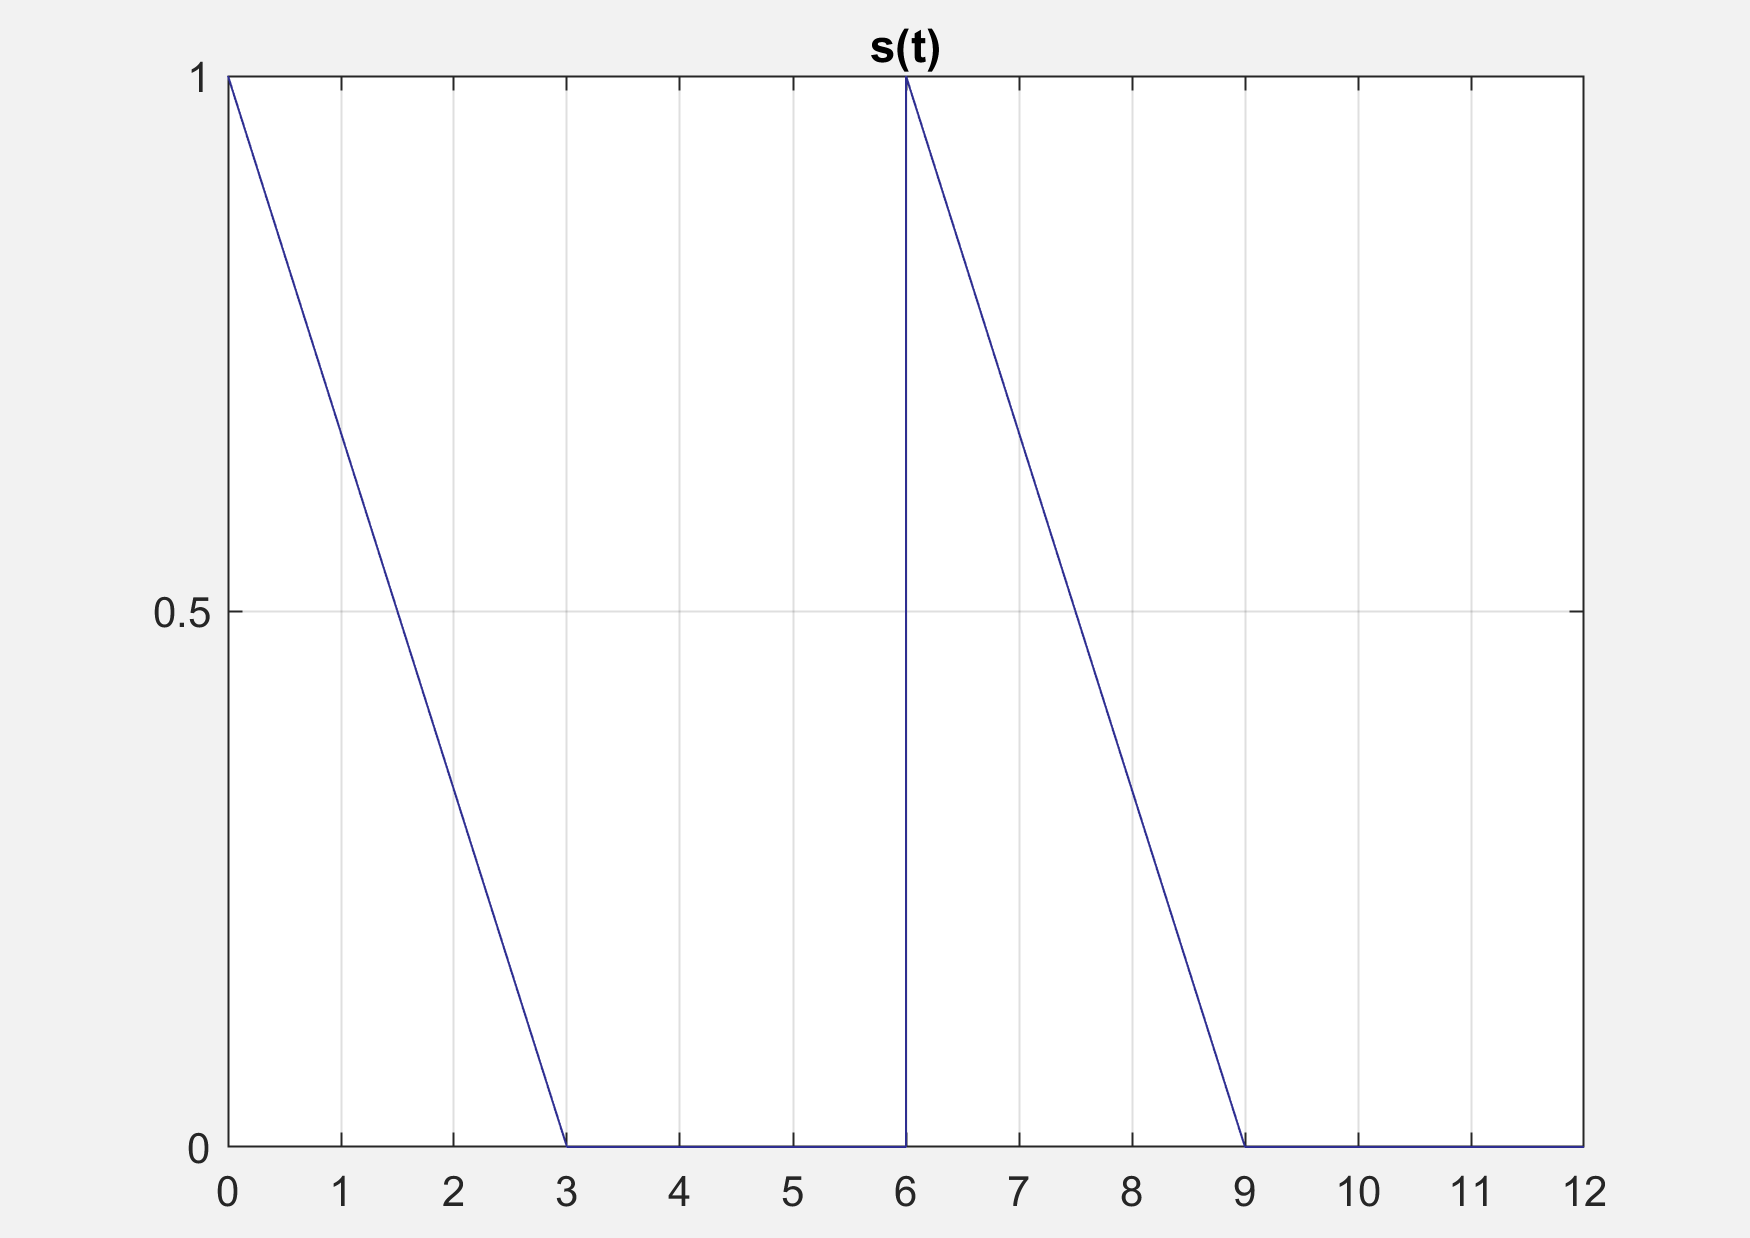
\includegraphics[width=\linewidth, keepaspectratio]{./assets/415.png}}
	}
\end{enumerate}

\section{Parameter of a periodic signal - A (4.1.6)}
Given is the periodic signal curve $s(t)$

\begin{figure}[H]
	\centering
	\begin{tikzpicture}
		\pgfplotsset{
			every axis plot/.append style={line width=1pt, mark=none}
		}
		\begin{axis}[
			clip=false,
			axis lines=middle,
			xmin=-0.5, xmax=12.5,
			xlabel={$t$},
			xmajorticks=false,
			ymin=-1.3, ymax=1.3,
			y=2.5cm,
			ylabel={$s(t)$},
			yticklabels={$\hat{s}$, $-\hat{s}$},
			ytick={1,-1},
			width=12cm,
			x label style={at={(current axis.right of origin)},	anchor=east, right=1mm},
			y label style={at={(current axis.above origin)}, anchor=south }
		]
			\addplot [samples=500, color=blue, domain=0:3.7*pi] {sin(deg(1.22*x))};
			
			% Nullstelle ist 0 + T*n / 2
			% T = 2*pi/1.22
			\draw[color=gray!80, line width=0.75pt, dashed] (2*pi/1.22, 0) -- (2*pi/1.22, 1.5);
			
			\draw[color=gray!80, line width=0.75pt, dashed] (2*pi/1.22/2*4, 0) -- (2*pi/1.22/2*4, 1.5);
			
			\draw[color=gray!80, line width=0.75pt, dashed] (2*pi/1.22/2*3, 0) -- (2*pi/1.22/2*3, 1.2);
			
			\draw[<->, color=gray!80, line width=0.75pt] (2*pi/1.22/2*2, 1.4) -- (2*pi/1.22/2*4, 1.4) node[midway, above] {\tiny $T_0$};
		\end{axis}
	\end{tikzpicture}
	\caption{\label{fig:416a}Characteristics of a periodic signal $s(t)$}
\end{figure}

\begin{enumerate}
	\item Rectified value(Gleichrichtwert) of the sinusoidal alternating voltage\newline
	In general, the rectification value(Gleichrichtwert) $\overline{\abs{s}}$ for a sinusoidal AC voltage describes an average value over the period duration that the signal generates after negative half-waves have been removed.
	\begin{equation*}
		\overline{\abs{s}} = \frac{1}{T_0}\int_{t_0}^{t_0+T_0}\abs{s(t)}\D{t}=\frac{1}{T_0}\int_{t_0}^{t_0+T_0}\abs{\hat{s}\cdot\sin\left(\omega_0\cdot{t}\right)}\D{t}
	\end{equation*}
	
	Calculation of the rectification value for $T_0=2\pi$, $\hat{s} = \mathrm{const.} = 1$
	\begin{figure}[H]
		\centering
		\begin{tikzpicture}
			\pgfplotsset{
				every axis plot/.append style={line width=1pt, mark=none}
			}
			\begin{axis}[
				clip=false,
				axis lines=middle,
				xmin=-0.5, xmax=12.5,
				xlabel={$t$},
				xmajorticks=false,
				ymin=-1.3, ymax=1.3,
				y=2.5cm,
				ylabel={$s(t)$},
				yticklabels={$\hat{s}$, $-\hat{s}$},
				ytick={1,-1},
				width=12cm,
				x label style={at={(current axis.right of origin)},	anchor=east, right=1mm},
				y label style={at={(current axis.above origin)}, anchor=south }
			]
				\addplot [name path=f1, samples=500, color=blue, domain=0:3.7*pi, restrict y to domain=0:1] {sin(deg(1.22*x))};
				\addplot [samples=500, color=blue!60, domain=0:3.7*pi, restrict y to domain=-1:0, dashed] {sin(deg(1.22*x))};
				\addplot [name path=f2, samples=500, color=blue, domain=0:3.7*pi, restrict y to domain=0:1] {sin(deg(1.22*x+pi))};
				
				\path[name path=axis] (axis cs:2*pi/1.22/2*2,0) -- (axis cs:2*pi/1.22/2*4,0);
				
				\addplot [thick, color=blue, fill=blue, fill opacity=0.05]
					fill between[of=f1 and axis, soft clip={domain=2*pi/1.22/2*2:2*pi/1.22/2*4}];
				\addplot [thick, color=blue, fill=blue, fill opacity=0.05]
					fill between[of=f2 and axis, soft clip={domain=2*pi/1.22/2*2:2*pi/1.22/2*4}];
				
				% Nullstelle ist 0 + T*n / 2
				% T = 2*pi/1.22
				\draw[color=gray!80, line width=0.75pt, dashed] (2*pi/1.22, 0) -- (2*pi/1.22, 1.5);
				
				\draw[color=gray!80, line width=0.75pt, dashed] (2*pi/1.22/2*4, 0) -- (2*pi/1.22/2*4, 1.5);
				
				\draw[color=gray!80, line width=0.75pt, dashed] (2*pi/1.22/2*3, 0) -- (2*pi/1.22/2*3, 1.2);
				
				\draw[<->, color=gray!80, line width=0.75pt] (2*pi/1.22/2*2, 1.4) -- (2*pi/1.22/2*4, 1.4) node[midway, above] {\tiny $T_0$};
			\end{axis}
		\end{tikzpicture}
		\caption{\label{fig:416b}Rectified signal $s_g(t)$ from figure ~\ref{fig:416a}, with integral areas}
	\end{figure}
	From figure ~\ref{fig:416b} it can be deduced that it is sufficient for the calculation to integrate over half a period and multiply this result by 2, as there are two positive half-waves in one period due to the rectification. This eliminates the amounts(Beträge) in the integral and the antiderivative(Stammfunktion) can be formed. Furthermore, the following generally applies to the circular frequency $\omega_0 = 2\pi/T_0.$
	{
		\setlength{\abovedisplayskip}{6pt}
		\setlength{\belowdisplayskip}{12pt}
		\begin{flalign*}
			\overline{\abs{s}} &= \frac{1}{T_0}\cdot2\int_{0}^{\frac{T_0}{2}}{s(t)}\D{t}
			=\frac{1}{T_0}\cdot2\int_{0}^{\frac{T_0}{2}}\hat{s}\cdot\sin\left(\omega_0\cdot{t}\right)\D{t}
			=\frac{2\hat{s}}{T_0}\int_{0}^{\frac{T_0}{2}}\sin\left(\omega_0\cdot{t}\right)\D{t} & \\
			& = \frac{2\hat{s}}{T_0}\cdot\left[\frac{-\cos\left(\omega_0\cdot{t}\right)}{\omega_0}\right]_0^{\frac{T_0}{2}}
			= \frac{\cancel{2}\hat{s}}{\bcancel{T_0}}\cdot\left[\frac{-\cos\left(\frac{2\pi}{T_0}t\right)}{\frac{\cancel{2}\pi}{\bcancel{T_0}}}\right]_0^{\frac{T_0}{2}} & \\
			& = \frac{\hat{s}}{\pi}\left(-\cos\left(\frac{\cancel{2}\pi}{\bcancel{T_0}}\cdot\frac{\bcancel{T_0}}{\cancel{2}}\right)+\cos\left(\frac{2\pi}{T_0}\cdot0\right)\right)
			= \frac{\hat{s}}{\pi} \left(-\cos\left(\pi\right)+\cos(0)\right) & \\
			& = \frac{2\hat{s}}{\pi} \approx \num{0,636}\overline{6}\;\hat{s}
		\end{flalign*}
	}
	\clearpage
	\item Description and representation of the curve and rectified value in Matlab
	\lstinputlisting[language=Matlab]{./assets/Lab1_416.m}
	{
		\setlength{\fboxsep}{0pt}%  
		\colorbox{backcolor}{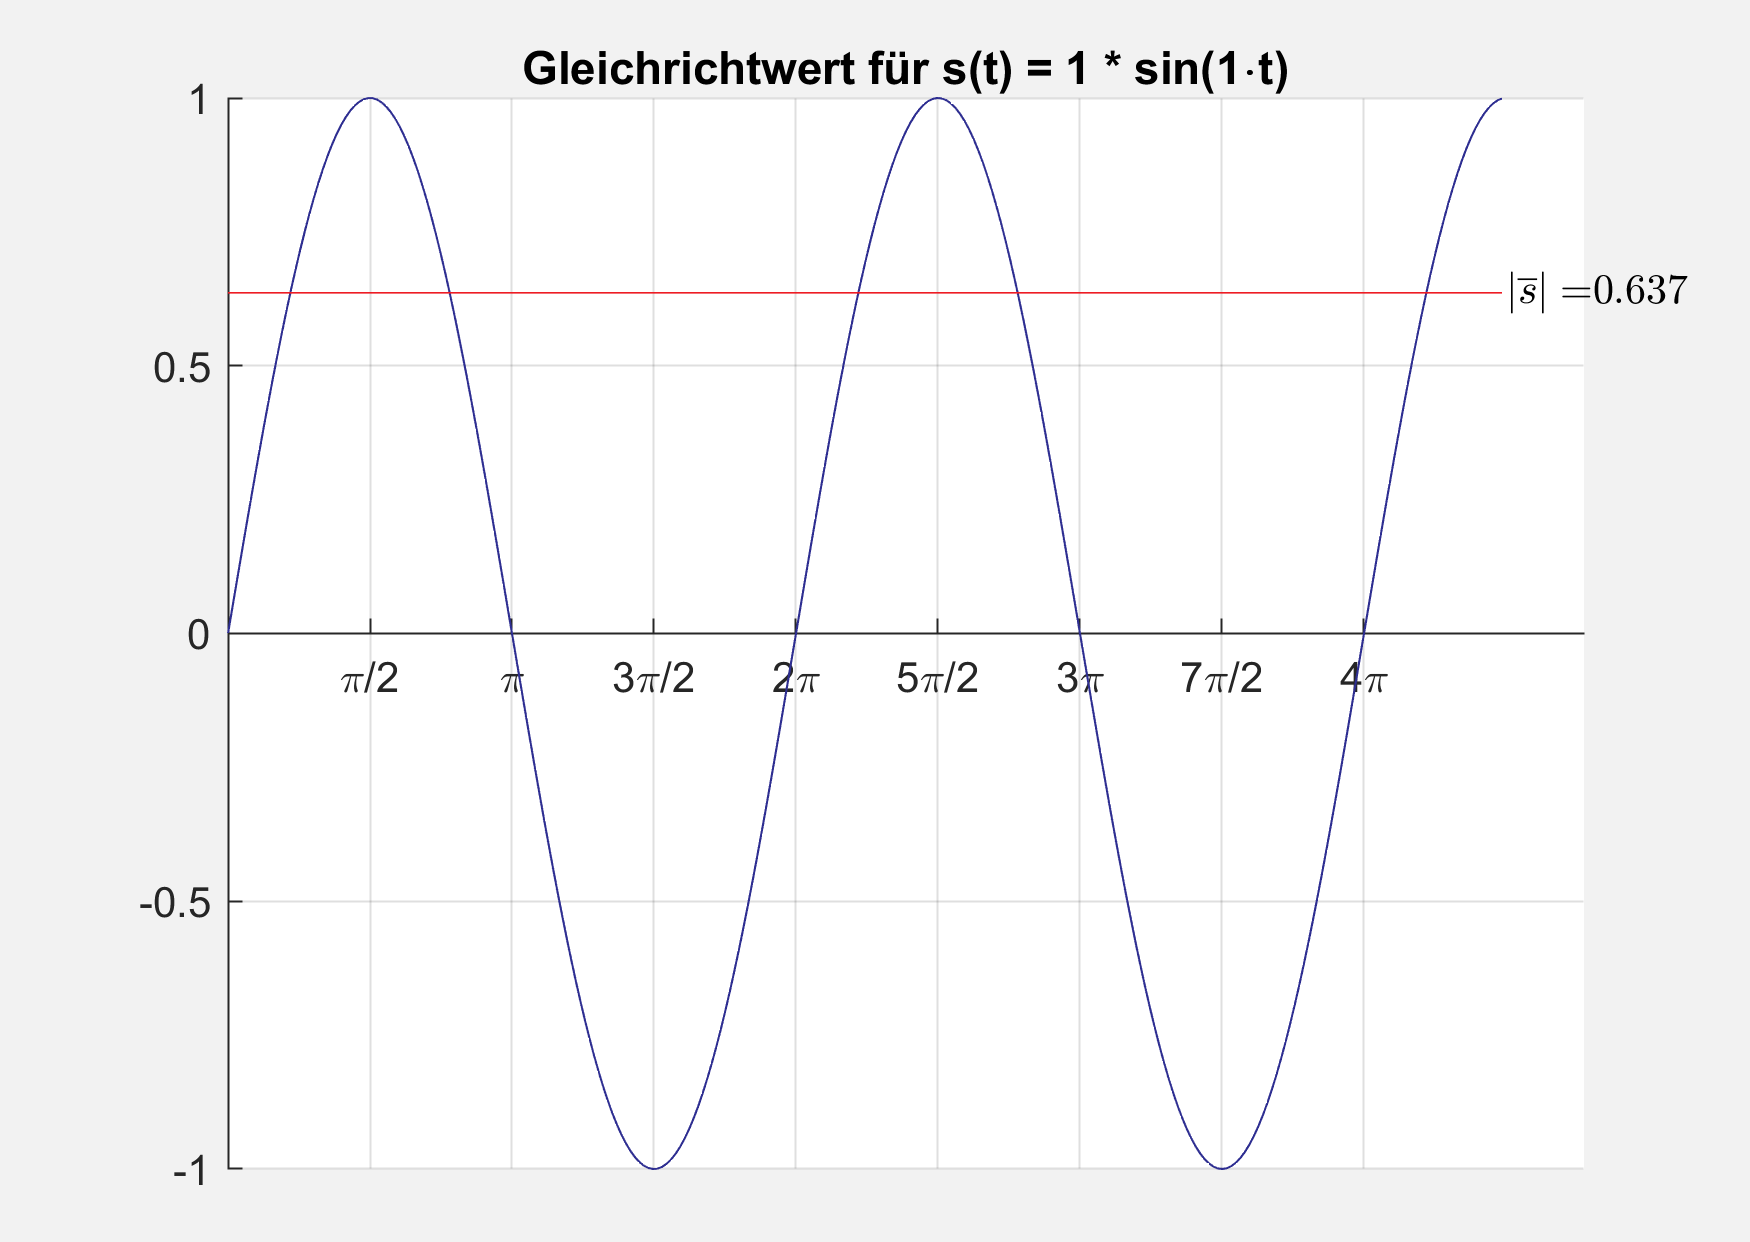
\includegraphics[width=\linewidth, keepaspectratio]{./assets/416.png}}
	}
\end{enumerate}

\section{Parameter of a periodic signal - B (4.1.7)}
Given is the periodic signal curve $s(t)$, so that ${s_g}_0=\sqrt{3}/2$ and $\hat{s}_0=1$ applies

\begin{figure}[H]
	\centering
	\begin{tikzpicture}
		\pgfplotsset{
			every axis plot/.append style={line width=1pt, mark=none}
		}
		\begin{axis}[
			clip=false,
			axis lines=middle,
			xmin=-0.5, xmax=4.5*pi,
			xlabel={$t$},
			xmajorticks=false,
			ymajorticks=false,
			ymin=-0.3,ymax=3,
			y=1.5cm,
			ylabel={$s(t)$},
			width=12cm,
			x label style={at={(current axis.right of origin)},	anchor=east, right=1mm},
			y label style={at={(current axis.above origin)}, anchor=south },
		]
			\addplot [samples=500, color=blue, domain=0:4.5*pi] {1*sin(deg(x))+sqrt(3)/2};
			\draw[color=gray!80, line width=0.75pt, dashed] (-0.2, {sqrt(3)/2}) -- (4.5*pi, {sqrt(3)/2});
			\draw[color=gray!80] node[left] at (-0.2,{sqrt(3)/2}) {\tiny ${s_g}_0$};
			
			\draw[color=gray!80, line width=0.75pt, dashed] (2*pi, 0) -- (2*pi, {sqrt(3)/2+1.3});
			\draw[color=gray!80, line width=0.75pt, dashed] (4*pi, 0) -- (4*pi, {sqrt(3)/2+1.3});
			\draw[<->, color=gray!80, line width=0.75pt] (2*pi, {sqrt(3)/2+1.3}) -- (4*pi, {sqrt(3)/2+1.3}) node[midway, above] {\tiny $T_0$};
			{1*sin(deg(x))+sqrt(3)/2}
			
			\draw[<->, color=gray!80, line width=0.75pt] (pi/2, {sqrt(3)/2}) -- (pi/2, {1*sin(deg(pi/2))+sqrt(3)/2}) node[midway, left] {\tiny $\hat{s}$};
			
		\end{axis}
	\end{tikzpicture}
	\caption{\label{fig:417}Characteristics of a periodic signal $s(t)$ with offset}
\end{figure}

The following applies for all calculations:
\begin{equation*}
	s(t) =\hat{s}\cdot\sin\left({\omega_0t}\right)+ s_{g_0}=
	1\cdot\sin\left({\omega_0t}\right)+\frac{\sqrt{3}}{2}
\end{equation*}

\begin{enumerate}
	\item Mean(Gleichwert) of the sinusoidal alternating variable
	From a mathematical point of view, the offset results in areas of different sizes when integrating over the period duration $T_0$ between the signal and the time axis.
	
	\begin{figure}[H]
		\centering
		\begin{tikzpicture}[line cap=rect]
			\pgfplotsset{
				every axis plot/.append style={line width=1pt, mark=none}
			}
			\begin{axis}[
				clip=false,
				axis lines=middle,
				xmin=-0.5, xmax=4.5*pi,
				xlabel={$t$},
				xmajorticks=false,
				ymajorticks=false,
				ymin=-0.3,ymax=3,
				y=1.5cm,
				ylabel={$s(t)$},
				width=12cm,
				x label style={at={(current axis.right of origin)},	anchor=east, right=1mm},
				y label style={at={(current axis.above origin)}, anchor=south },
			]
				\addplot [name path=positive, samples=500, color=green, domain=2*pi:4*pi, restrict y to domain=0:5] {sin(deg(x))+sqrt(3)/2};
				\addplot [name path=negative, samples=500, color=red, domain=2*pi:4*pi, restrict y to domain=-1:0] {sin(deg(x))+sqrt(3)/2};
				
				\path[name path=axis] (axis cs:0,0) -- (axis cs:4.5*pi,0);
				\addplot [fill=red, fill opacity=0.05]
					fill between[of=negative and axis, soft clip={domain=2*pi:4*pi}];
					
					
				\addplot [fill=green, fill opacity=0.05]
					fill between[of=positive and axis, soft clip={domain=2*pi:4*pi}];
					
				\addplot [samples=500, color=blue, domain=0:2*pi] {sin(deg(x))+sqrt(3)/2};
				\addplot [samples=500, color=blue, domain=4*pi:4.5*pi] {sin(deg(x))+sqrt(3)/2};
				
				
				\draw[color=gray!80, line width=0.75pt, dashed] (-0.2, {sqrt(3)/2}) -- (4.5*pi, {sqrt(3)/2});
				\draw[color=gray!80] node[left] at (-0.2,{sqrt(3)/2}) {\tiny ${s_g}_0$};
				\draw[color=gray!80, line width=0.75pt, dashed] (2*pi, 0) -- (2*pi, {sqrt(3)/2+1.3});
				\draw[color=gray!80, line width=0.75pt, dashed] (4*pi, 0) -- (4*pi, {sqrt(3)/2+1.3});
				\draw[<->, color=gray!80, line width=0.75pt] (2*pi, {sqrt(3)/2+1.3}) -- (4*pi, {sqrt(3)/2+1.3}) node[midway, above] {\tiny $T_0$};
				{1*sin(deg(x))+sqrt(3)/2}
				
				\draw[<->, color=gray!80, line width=0.75pt] (pi/2, {sqrt(3)/2}) -- (pi/2, {1*sin(deg(pi/2))+sqrt(3)/2}) node[midway, left] {\tiny $\hat{s}$};
				
			\end{axis}
		\end{tikzpicture}
		\captionsetup{format=hang,justification=raggedright}
		\caption{\label{fig:417a}Signal $s(t)$ with integration areas\\(green - positive component; - red negative component)}
	\end{figure}
	

	\begin{equation*}
		\overline{s} = \frac{1}{T_0}\int_{t_0}^{t_0+T_0}s(t)\D{t}
	\end{equation*}
	{
		\setlength{\abovedisplayskip}{6pt}
		\setlength{\belowdisplayskip}{12pt}
		\begin{flalign*}
			\overline{s} &=\frac{1}{T_0}\int_{0}^{T_0}{s(t)}\D{t}
			= \frac{1}{T_0}\int_{0}^{T_0}\sin({\omega_0t})+\frac{\sqrt{3}}{2}\D{t} & \\
			& = \frac{1}{T_0}\int_{0}^{T_0}\sin({\omega_0t})\D{t} + \int_{0}^{T_0}\frac{\sqrt{3}}{2}\D{t} & \\
			& = \frac{1}{T_0} \left(\frac{1}{\omega_0}\Big[-\cos(\omega_0t)\Big]_0^{T_0} + \left[\frac{\sqrt{3}}{2}t\right]_0^{T_0} \right) & \\
			& = \frac{1}{\cancel{T_0}} \frac{1}{\frac{2\pi}{\cancel{T_0}}}\left[-\cos\left(\frac{2\pi}{\cancel{T_0}}\cancel{T_0}\right)-\big(-\cos(0)\big)\right]
			+ \frac{1}{\cancel{T_0}} \left[\frac{\sqrt{3}}{2}\cancel{T_0}-\frac{\sqrt{3}}{2}\cdot0\right] & \\
			& = \frac{1}{2\pi}\left[-\cos\left(2\pi\right)+\cos(0)\right]
			+ \frac{\sqrt{3}}{2} & \\
			& = \frac{\sqrt{3}}{2} & 
		\end{flalign*}
	}
	
	\item Average absolute value <AAV>(Gleichrichtwert) of the sinusoidal alternating variable
	\begin{equation*}
		\overline{\abs{s}} = \frac{1}{T_0}\int_{t_0}^{t_0+T_0}\abs{s(t)}\D{t}
	\end{equation*}	
	The following rectified signal results from Figure ~\ref{fig:417a} after rectification due to the asymmetrical distribution around the time axis
	
	\begin{figure}[H]
		\centering
		\begin{tikzpicture}[line cap=rect]
			\pgfplotsset{
				every axis plot/.append style={line width=1pt, mark=none}
			}
			\begin{axis}[
				clip=false,
				axis lines=middle,
				xmin=-0.5, xmax=4.5*pi,
				xlabel={$t$},
				xmajorticks=false,
				ymajorticks=false,
				ymin=-0.3,ymax=3,
				y=1.5cm,
				ylabel={$s(t)$},
				width=12cm,
				x label style={at={(current axis.right of origin)},	anchor=east, right=1mm},
				y label style={at={(current axis.above origin)}, anchor=south },
			]
				\addplot [name path=f1, samples=500, color=blue, domain=0:4.5*pi, restrict y to domain=0:5] {sin(deg(x))+sqrt(3)/2};
				\addplot [samples=500, color=blue!60, domain=0:4.5*pi, restrict y to domain=-1:0, dashed] {sin(deg(x))+sqrt(3)/2};
				\addplot [name path=f2, samples=500, color=blue, domain=0:4.5*pi, restrict y to domain=0:1] {sin(-deg(x))+sqrt(3)/2*-1};
			
				\path[name path=axis] (axis cs:0,0) -- (axis cs:4.5*pi,0);
				\addplot [fill=blue, fill opacity=0.05]
					fill between[of=f1 and axis, soft clip={domain=2*pi:4*pi}];
					
				\addplot [fill=blue, fill opacity=0.05]
					fill between[of=f2 and axis, soft clip={domain=2*pi:4*pi}];
				
				\draw[color=gray!80, line width=0.75pt, dashed] (-0.2, {sqrt(3)/2}) -- (4.5*pi, {sqrt(3)/2});
				\draw[color=gray!80] node[left] at (-0.2,{sqrt(3)/2}) {\tiny ${s_g}_0$};
				
				\draw[color=gray!80, line width=0.75pt, dashed] (2*pi, 0) -- (2*pi, {sqrt(3)/2+1.3});
				\draw[color=gray!80, line width=0.75pt, dashed] (4*pi, 0) -- (4*pi, {sqrt(3)/2+1.3});
				\draw[<->, color=gray!80, line width=0.75pt] (2*pi, {sqrt(3)/2+1.3}) -- (4*pi, {sqrt(3)/2+1.3}) node[midway, above] {\tiny $T_0$};
				
				\draw[<->, color=gray!80, line width=0.75pt] (pi/2, {sqrt(3)/2}) -- (pi/2, {1*sin(deg(pi/2))+sqrt(3)/2}) node[midway, left] {\tiny $\hat{s}$};
			\end{axis}
		\end{tikzpicture}
		\caption{\label{fig:417b}Rectified signal $s(t)$}
	\end{figure}
	A closer look at Figure ~\ref{fig:417b} reveals two integration areas in the $T_0$ range. These become clear when the period is shifted to the intersection points of the rectified signal components (zero crossing).	
	\begin{figure}[H]
		\centering
		\begin{tikzpicture}[line cap=rect]
			\pgfplotsset{
				every axis plot/.append style={line width=1pt, mark=none}
			}
			\begin{axis}[
				clip=false,
				axis lines=middle,
				xmin=-0.5, xmax=4.5*pi,
				xlabel={$t$},
				xmajorticks=false,
				ymajorticks=false,
				ymin=-0.3,ymax=3,
				y=1.5cm,
				ylabel={$s(t)$},
				width=12cm,
				x label style={at={(current axis.right of origin)},	anchor=east, right=1mm},
				y label style={at={(current axis.above origin)}, anchor=south },
			]
			
				\addplot [samples=500, color=blue, domain=0:{2*pi - rad(asin(sqrt(3)/2))}, restrict y to domain=0:5] {sin(deg(x))+sqrt(3)/2};
				\addplot [samples=500, color=blue, domain={4*pi - rad(asin(sqrt(3)/2))}:{4.5*pi}, restrict y to domain=0:5] {sin(deg(x))+sqrt(3)/2};
				\addplot [samples=500, color=blue!60, domain=0:4.5*pi, restrict y to domain=-1:0, dashed] {sin(deg(x))+sqrt(3)/2};
				\addplot [samples=500, color=blue, domain=0:{2*pi - rad(asin(sqrt(3)/2))}, restrict y to domain=0:1] {sin(-deg(x))+sqrt(3)/2*-1};
				\addplot [samples=500, fill=blue, fill opacity=0.05, color=blue, domain={2*pi - rad(asin(sqrt(3)/2))}:{4*pi - rad(asin(sqrt(3)/2))}, restrict y to domain=0:5] {sin(deg(x))+sqrt(3)/2};
				
				\addplot [samples=500, fill=blue, fill opacity=0.05, draw=blue, domain={2*pi - rad(asin(sqrt(3)/2))}:{4*pi - rad(asin(sqrt(3)/2))}, restrict y to domain=0:1] {sin(-deg(x))+sqrt(3)/2*-1};
				
				\draw[color=gray!80, line width=0.75pt, dashed] (-0.2, {sqrt(3)/2}) -- (4.5*pi, {sqrt(3)/2});
				\draw[color=gray!80] node[left] at (-0.2,{sqrt(3)/2}) {\tiny ${s_g}_0$};
				
				\draw[color=gray!80, line width=0.75pt, dashed]
					({2*pi - rad(asin(sqrt(3)/2))}, 0) -- ({2*pi - rad(asin(sqrt(3)/2))}, {sqrt(3)/2+1.3});
				\draw[color=gray!80, line width=0.75pt, dashed]
					({4*pi - rad(asin(sqrt(3)/2))}, 0) -- ({4*pi - rad(asin(sqrt(3)/2))}, {sqrt(3)/2+1.3});
				\draw[<->, color=gray!80, line width=0.75pt]
					({2*pi - rad(asin(sqrt(3)/2))}, {sqrt(3)/2+1.3}) -- ({4*pi - rad(asin(sqrt(3)/2))}, {sqrt(3)/2+1.3}) node[midway, above] {\tiny $T_0$};
				
				\draw[<->, color=gray!80, line width=0.75pt]
					(pi/2, {sqrt(3)/2}) -- (pi/2, {sin(deg(pi/2))+sqrt(3)/2}) node[midway, left] {\tiny $\hat{s}$};
				
				\node at ({2*pi - rad(asin(sqrt(3)/2))}, 0)[below=3pt] {$t_1$};
				\node at ({4*pi - rad(asin(sqrt(3)/2)) - sqrt(3)/2)}, 0)[below=3pt] {$t_2$};
				\node at ({4*pi - rad(asin(sqrt(3)/2))}, 0)[below=3pt] {$t_3$};
					
			\end{axis}
		\end{tikzpicture}
		\captionsetup{justification=centering}
		\caption{\label{fig:417c}Rectified signal $s(t)$\\with shifted period duration in the zero crossings}
	\end{figure}
	
	\underline{Zero point calculation:}\\
	\begin{tabularx}{\linewidth}{rlll}
		$s(t)$ & $=$ & $0$ & \\[1.5ex]
		$\sin(\omega_0\cdot{t}) + \dfrac{\sqrt{3}}{2}$ & $=$ & $0$ & $\quad \left|\;- \dfrac{\sqrt{3}}{2}\right. $ \\[1.5ex]
		$\sin(\omega_0\cdot{t})$ & $=$ & $-\dfrac{\sqrt{3}}{2}$    & $\quad \left|\; \Rightarrow \omega_0\cdot{t_2} = \dfrac{4\pi}{3}\;\right.$ \\[1.5ex]
		&&& \phantom{$\quad |\;\Rightarrow$}$\omega_0\cdot{t_3} = \dfrac{5\pi}{3}$  \\[1.5ex]
		&&& \phantom{$\quad |\;\Rightarrow$}(from unit circle) \\[1.5ex]
	\end{tabularx}
	
	\underline{Calculation of the integral:}\\
	
	
	
	
%	{
%		\setlength{\abovedisplayskip}{6pt}
%		\setlength{\belowdisplayskip}{12pt}
%		\begin{flalign*}
%			\overline{s} &=\frac{1}{T_0}\int_{0}^{T_0}{s(t)}\D{t}
%			= \frac{1}{T_0}\int_{0}^{T_0}\sin({\omega_0t})+\frac{\sqrt{3}}{2}\D{t} & \\
%			& = \frac{1}{T_0}\int_{0}^{T_0}\sin({\omega_0t})\D{t} + \int_{0}^{T_0}\frac{\sqrt{3}}{2}\D{t} & \\
%			& = \frac{1}{T_0} \left(\frac{1}{\omega_0}\Big[-\cos(\omega_0t)\Big]_0^{T_0} + \left[\frac{\sqrt{3}}{2}t\right]_0^{T_0} \right) & \\
%			& = \frac{1}{\cancel{T_0}} \frac{1}{\frac{2\pi}{\cancel{T_0}}}\left[-\cos\left(\frac{2\pi}{\cancel{T_0}}\cancel{T_0}\right)-\big(-\cos(0)\big)\right]
%			+ \frac{1}{\cancel{T_0}} \left[\frac{\sqrt{3}}{2}\cancel{T_0}-\frac{\sqrt{3}}{2}\cdot0\right] & \\
%			& = \frac{1}{2\pi}\left[-\cos\left(2\pi\right)+\cos(0)\right]
%			+ \frac{\sqrt{3}}{2} & \\
%			& = \frac{\sqrt{3}}{2} & 
%		\end{flalign*}
%	}
%	
%	{
%		\setlength{\abovedisplayskip}{6pt}
%		\setlength{\belowdisplayskip}{12pt}
%		\begin{flalign*}
%			\overline{\abs{s}} &= \frac{1}{T_0}\cdot2\int_{0}^{\frac{T_0}{2}}{s(t)}\D{t}
%			=\frac{1}{T_0}\cdot2\int_{0}^{\frac{T_0}{2}}\hat{s}\cdot\sin\left(\omega_0\cdot{t}\right)\D{t}
%			=\frac{2\hat{s}}{T_0}\int_{0}^{\frac{T_0}{2}}\sin\left(\omega_0\cdot{t}\right)\D{t} & \\
%			& = \frac{2\hat{s}}{T_0}\cdot\left[\frac{-\cos\left(\omega_0\cdot{t}\right)}{\omega_0}\right]_0^{\frac{T_0}{2}}
%			= \frac{\cancel{2}\hat{s}}{\bcancel{T_0}}\cdot\left[\frac{-\cos\left(\frac{2\pi}{T_0}t\right)}{\frac{\cancel{2}\pi}{\bcancel{T_0}}}\right]_0^{\frac{T_0}{2}} & \\
%			& = \frac{\hat{s}}{\pi}\left(-\cos\left(\frac{\cancel{2}\pi}{\bcancel{T_0}}\cdot\frac{\bcancel{T_0}}{\cancel{2}}\right)+\cos\left(\frac{2\pi}{T_0}\cdot0\right)\right)
%			= \frac{\hat{s}}{\pi} \left(-\cos\left(\pi\right)+\cos(0)\right) & \\
%			& = \frac{2\hat{s}}{\pi} \approx \num{0,636}\overline{6}\;\hat{s}
%		\end{flalign*}
%	}
	
	\item Description and visualization in Matlab
	\lstinputlisting[language=Matlab]{./assets/Lab1_417.m}
	{
		\setlength{\fboxsep}{0pt}%  
		\colorbox{backcolor}{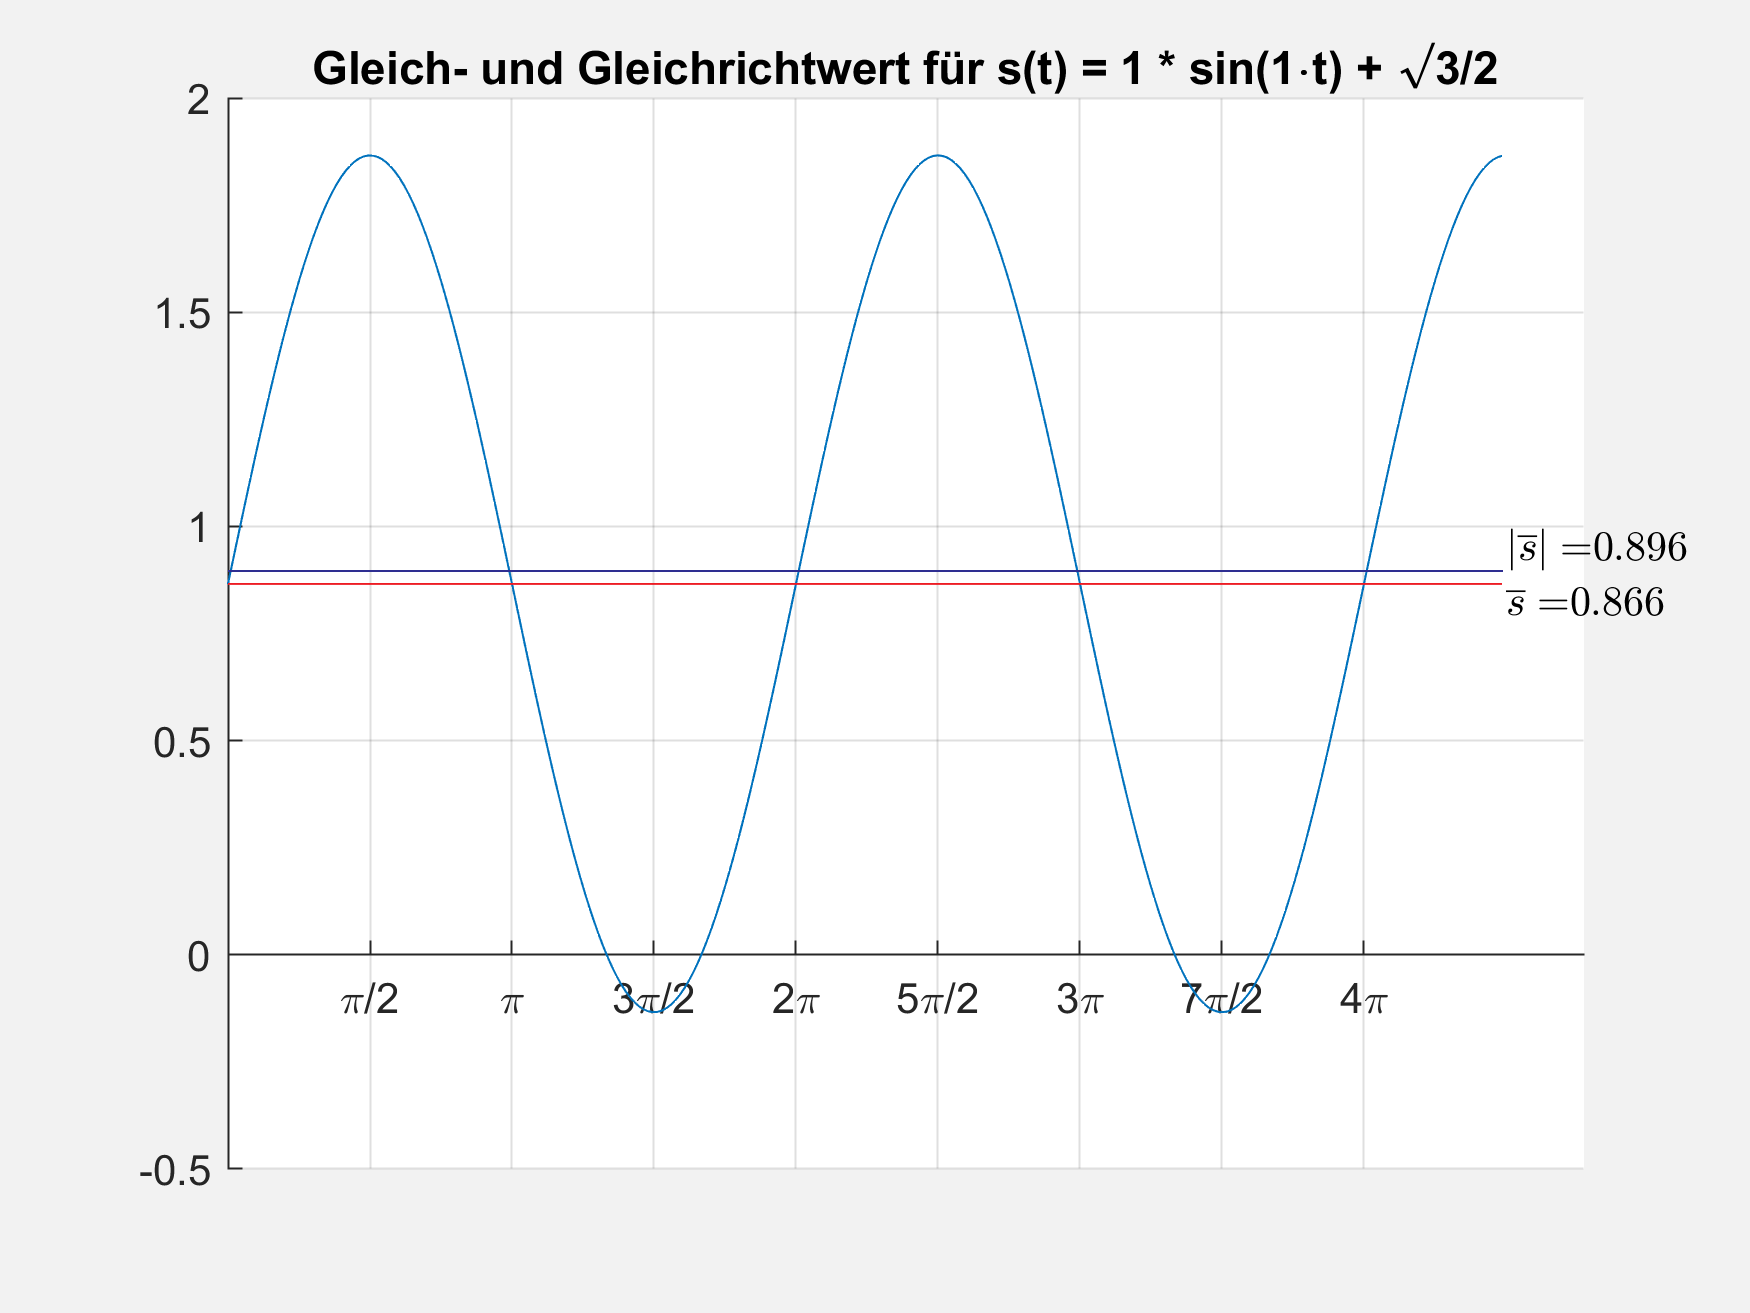
\includegraphics[width=\linewidth, keepaspectratio]{./assets/417.png}}
	}	
\end{enumerate}
\clearpage

\section{Discrete signals (4.1.8)}
Given is the discrete signal:
\begin{equation*}
	s[n] = \cos[\Omega_0\cdot(n+P_0)+\theta_0]
\end{equation*}

\begin{enumerate}
	\item Calculation of the period duration $N_0$ for the following cases:
	
	\begin{nscenter}
		\begin{tabular}{c|lll}
			& $\Omega_0$ & $P_0$ & $\theta_0$ \\
			\hline
			1 & $\pi/{3}$ & $0$ & $2\pi$ \\
			2 & $3\pi/4$ & $2$ & $\pi/4$ \\
			3 & $3/4$ & $1$ & $1/4$ 
		\end{tabular}
	\end{nscenter}
	
	The normalization rule $\Omega_0$ is used to normalize a fundamental frequency $f_0$ to the sampling frequency $f_s$.
	\begin{equation*}
		\Omega_0 = 2\pi\frac{f_0}{f_s}
	\end{equation*}
	Following the definition of the circular frequency for continuous signals, the quotient of the frequencies in the normalization rule can also be expressed with the period duration for discrete signals
	\begin{equation*}
		\omega_0 = \frac{2\pi}{T} \rightarrow \Omega_0 = \frac{2\pi}{N_0}
	\end{equation*}
	converted to $N_0$
	\begin{equation*}
		N_0 = \frac{2\pi}{\Omega_0}
	\end{equation*}
	Calculations:
	{
		\setlength{\abovedisplayskip}{4pt}
		\setlength{\belowdisplayskip}{6pt}
		\setlength{\abovedisplayshortskip}{0pt}
		\setlength{\belowdisplayshortskip}{0pt}
		\begin{flalign*}
			&N_{0_{1}} = \frac{2\pi}{\frac{\pi}{3}} = \frac{2\pi\cdot3}{\pi} = 6 &
			&N_{0_{2}} = \frac{2\pi}{\frac{3\pi}{4}} = \frac{2\pi\cdot4}{3\pi} = \frac{8}{3} &
			&N_{0_{3}} = \frac{2\pi}{\frac{3}{4}} =   \frac{2\pi\cdot4}{3} = \frac{8\pi}{3} & 
		\end{flalign*}
	}
	
	\item Given are the discrete signals:
	\begin{align*}
		s_x[n] = \cos[\Omega_x\cdot(n+P_x)+\theta_x] \\
		s_y[n] = \cos[\Omega_y\cdot(n+P_y)+\theta_y] \\
	\end{align*}
	and the parameters	
	\begin{nscenter}
		\begin{tabular}{c|lll|lll}
			& $\Omega_x$ & $P_x$ & $\theta_x$ 
			& $\Omega_y$ & $P_y$ & $\theta_y$ \\
			\hline
			1 & $\pi/{3}$ & $0$ & $2\pi$ 
			& $8\pi/{3}$ & $0$ & $0$ \\
			2 & $3\pi/4$ & $2$ & $\pi/4$
			& $3\pi/4$ & $1$ & $-\pi$ \\
			3 & $3/4$ & $1$ & $1/4$
			& $3/4$ & 0 & 1
		\end{tabular}
	\end{nscenter}
	
	We get the functions:
	{
		\setlength{\abovedisplayskip}{0pt}
		\setlength{\belowdisplayskip}{6pt}
		\setlength{\abovedisplayshortskip}{0pt}
		\setlength{\belowdisplayshortskip}{0pt}
		\begin{align*}
			s_{x_1}[n] = \cos\left[\frac{\pi}{3}\cdot\left(n-0\right)+2\pi\right] & \qquad 
			s_{y_1}[n] = \cos\left[\frac{8\pi}{3}\cdot\left(n-0\right)+0\right] \\
			%
			s_{x_2}[n] = \cos\left[\frac{3\pi}{4}\cdot\left(n-2\right)+\frac{\pi}{4}\right] & \qquad 
			s_{y_2}[n] = \cos\left[\frac{3\pi}{4}\cdot\left(n-1\right)-\pi\right] \\
			%
			s_{x_3}[n] = \cos\left[\frac{3}{4}\cdot\left(n-1\right)+\frac{1}{4}\right] & \qquad 
			s_{y_3}[n] = \cos\left[\frac{3}{4}\cdot\left(n-0\right)+1\right]
		\end{align*}
	}
	\subsubsection{Solution}
	The aim is to check for which of the given combination(s) it is true that $s_{x_i}[n]$ is identical to $s_{y_i}[n]$.
	
	{
		\setlength{\abovedisplayskip}{0pt}
		\setlength{\belowdisplayskip}{6pt}
		\setlength{\abovedisplayshortskip}{0pt}
		\setlength{\belowdisplayshortskip}{0pt}
		
		\underline{Signal combination 1:}
		
		\begin{minipage}[t]{0.499999\linewidth}
			\begin{flalign*}
				s_{x_1}[n] & = \cos\left[\frac{\pi}{3}\cdot\left(n-0\right)+2\pi\right] & \\
				&=\cos\left[\frac{\pi}{3}n+2\pi\right] & \\
				&=\cos\left[\frac{\pi}{3}n\right] &
			\end{flalign*}
		\end{minipage}
		\begin{minipage}[t]{0.499999\linewidth}
			\begin{flalign*}
				s_{y_1}[n] & = \cos\left[\frac{8\pi}{3}\cdot\left(n-0\right)+0\right] & \\
				&= \cos\left[\frac{8\pi}{3}n\right] &
			\end{flalign*}
		\end{minipage}
		\vspace{2pt} \\
		$\Rightarrow$ The signal combination has only the same amplitude, but differs in frequency.
		
		\vspace{4pt}
		\underline{Signal combination 2:}
		
		\begin{minipage}[t]{0.499999\linewidth}
			\begin{flalign*}
				s_{x_2}[n] &= \cos\left[\frac{3\pi}{4}\cdot\left(n-2\right)+\frac{\pi}{4}\right] & \\
				&=\cos\left[\frac{3\pi}{4}n - \frac{3\pi}{2} + \frac{\pi}{4}\right] & \\
				&=\cos\left[\frac{3\pi}{4}n - \frac{5\pi}{4}\right] &
			\end{flalign*}
		\end{minipage}
		\begin{minipage}[t]{0.499999\linewidth}
			\begin{flalign*}
				s_{y_2}[n] &= \cos\left[\frac{3\pi}{4}\cdot\left(n-1\right)-\pi\right] & \\
				&=\cos\left[\frac{3\pi}{4}n - \frac{3\pi}{4} - \pi\right] & \\
				&=\cos\left[\frac{3\pi}{4}n - \frac{7\pi}{4}\right] &
			\end{flalign*}
		\end{minipage}
		\vspace{2pt} \\
		$\Rightarrow$ The signal combination has the same frequency and amplitude, but differs by a phase shift of $\SI{90}{\degree}$, $\pi/2$.
		
		\vspace{4pt}
		\underline{Signal combination 3:}
		
		\begin{minipage}[t]{0.499999\linewidth}
			\begin{flalign*}
				s_{x_3}[n] &= \cos\left[\frac{3}{4}\cdot\left(n-1\right)+\frac{1}{4}\right] & \\
				&=\cos\left[\frac{3}{4}n - \frac{3}{4} + \frac{1}{4}\right] & \\
				&=\cos\left[\frac{3}{4}n - \frac{1}{2}\right] &
			\end{flalign*}
		\end{minipage}
		\begin{minipage}[t]{0.5\linewidth}
			\begin{flalign*}
				s_{y_3}[n] &= \cos\left[\frac{3}{4}\cdot\left(n-0\right)+1\right] & \\
				&=\cos\left[\frac{3}{4}n - 0 + 1\right] & \\
				&=\cos\left[\frac{3}{4}n + 1\right] &
			\end{flalign*}
		\end{minipage}
		\vspace{2pt} \\
		$\Rightarrow$ The signal combination has the same frequency and amplitude, but has a phase shift of $\SI{0,5}{\radian}$.
	}	
\end{enumerate}
\clearpage

\section{Pulse sequences - Matlab/Simulink (4.1.9)}
Using Matlab, the following discrete-time pulse sequences are to be visualized in the time range of $n \in [-20,20]$

\begin{flalign*}
	s_1[n]&=\delta[n]\quad\textrm{(Dirac delta function)} \\
	s_2[n]&=\sigma[n]\quad\textrm{(snap-action function(Sprungfunktion))} \\
	s_3[n]&=\begin{cases}
		0,\: \textrm{für} \quad n \leq 0 \\
		n,\: \textrm{für} \quad n > 0
	\end{cases} \\
	s_4[n]&=\begin{cases}
		-2,&\: \textrm{für} \quad n \leq -2 \\
		n,&\: \textrm{für} \quad -2 < n < 2 \\
		2,&\: \textrm{für} \quad n \geq 2
	\end{cases}
\end{flalign*}

\lstinputlisting[language=Matlab]{./assets/Lab1_419.m}
{
	\setlength{\fboxsep}{0pt}%  
	\colorbox{backcolor}{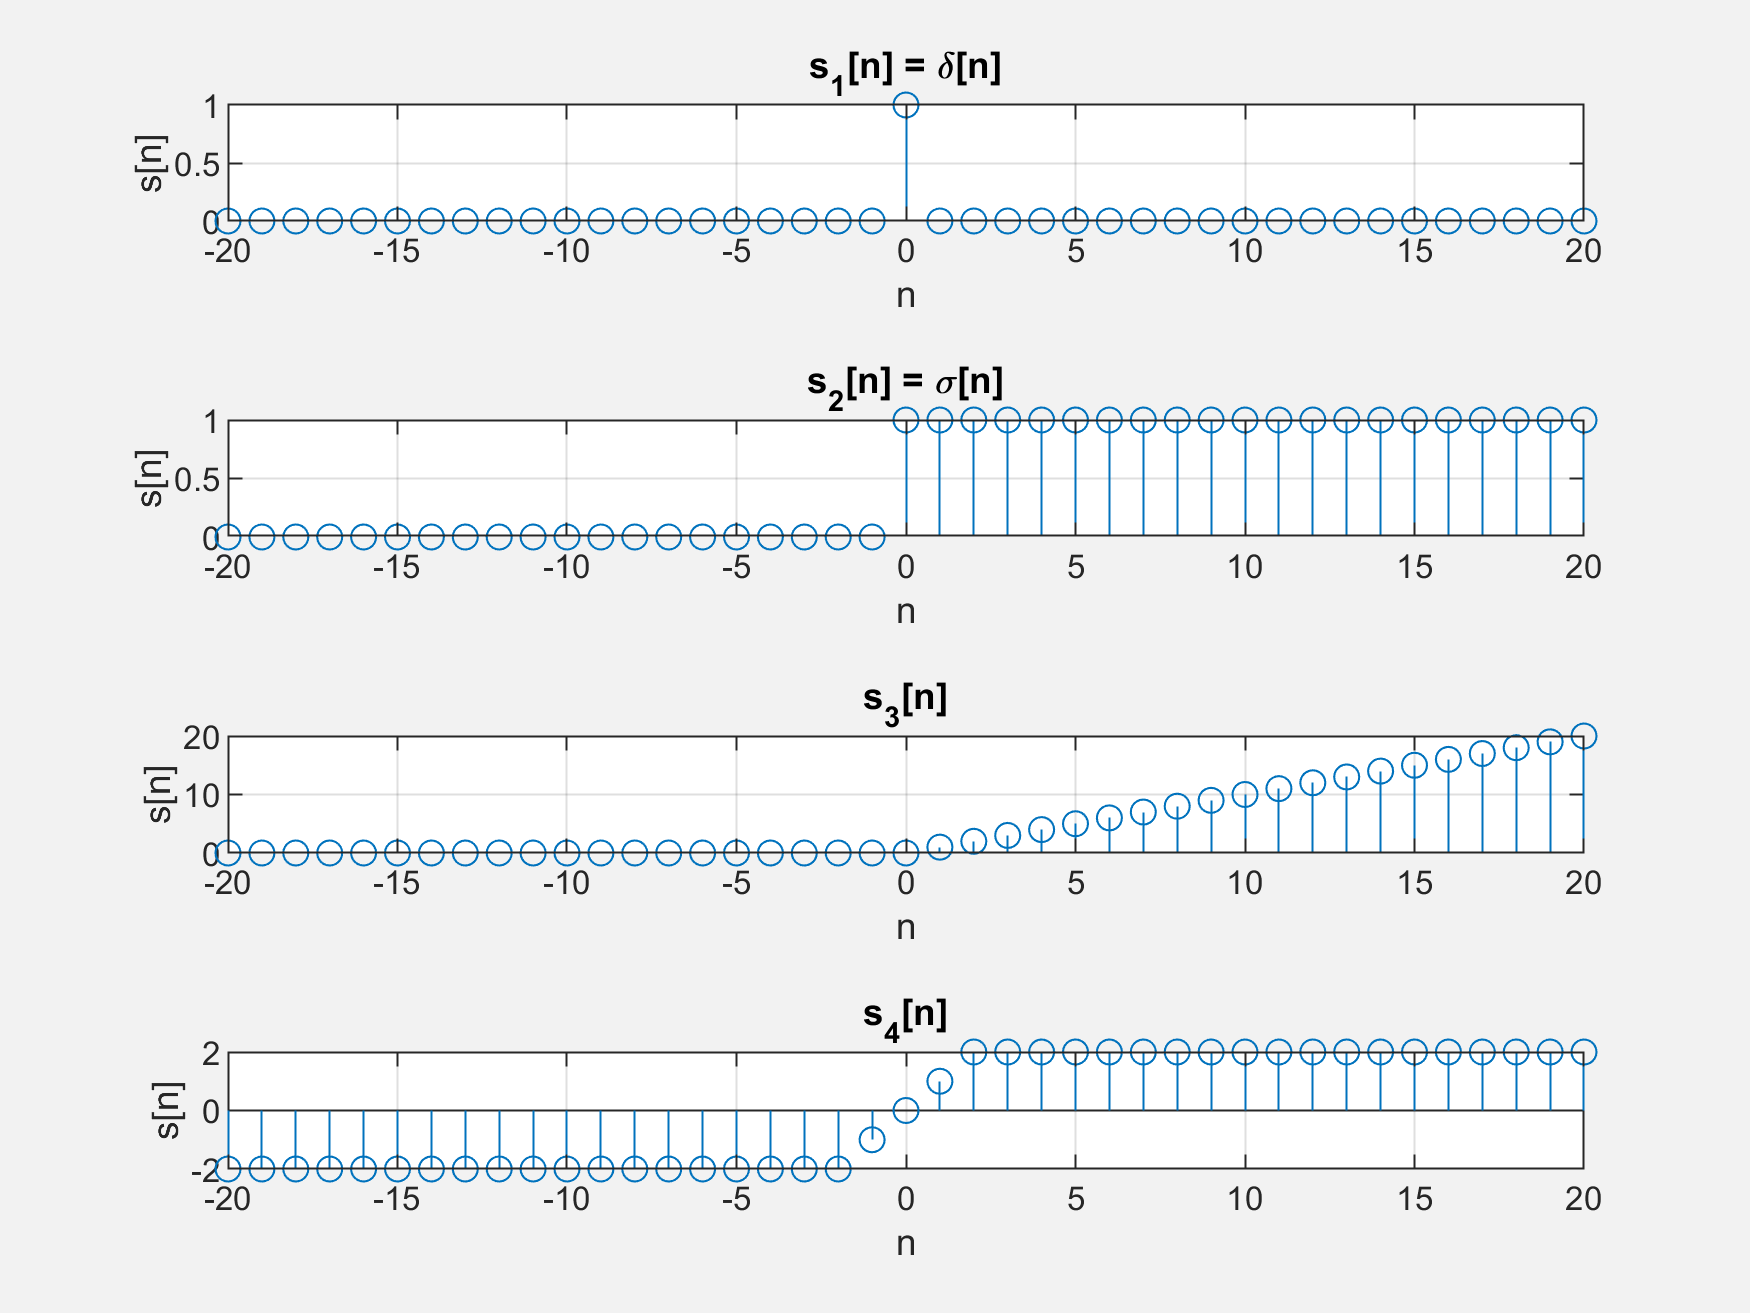
\includegraphics[width=\linewidth, keepaspectratio]{./assets/419.png}}
}

\end{document}